\documentclass[c]{beamer}  % [t], [c], или [b] --- вертикальное выравнивание на слайдах (верх, центр, низ)
%\documentclass[handout]{beamer} % Раздаточный материал (на слайдах всё сразу)
%\documentclass[aspectratio=169]{beamer} % Соотношение сторон

%\usetheme{Berkeley} % Тема оформления
%\usetheme{Bergen}
%\usetheme{Szeged}

%\usecolortheme{beaver} % Цветовая схема
%\useinnertheme{circles}
%\useinnertheme{rectangles}

\usetheme{MIET}

%%% Работа с русским языком
\usepackage{cmap}					% поиск в PDF
\usepackage{mathtext} 				% русские буквы в формулах
\usepackage[T2A]{fontenc}			% кодировка
\usepackage[utf8]{inputenc}			% кодировка исходного текста
\usepackage[english,russian]{babel}	% локализация и переносы

%% Beamer по-русски
\newtheorem{rtheorem}{Теорема}
\newtheorem{rproof}{Доказательство}
\newtheorem{rexample}{Пример}

%%% Дополнительная работа с математикой
\usepackage{amsmath,amsfonts,amssymb,amsthm,mathtools} % AMS
\usepackage{icomma} % "Умная" запятая: $0,2$ --- число, $0, 2$ --- перечисление

%% Номера формул
%\mathtoolsset{showonlyrefs=true} % Показывать номера только у тех формул, на которые есть \eqref{} в тексте.
%\usepackage{leqno} % Нумерация формул слева

%% Свои команды
\DeclareMathOperator{\sgn}{\mathop{sgn}}

%% Перенос знаков в формулах (по Львовскому)
\newcommand*{\hm}[1]{#1\nobreak\discretionary{}
	{\hbox{$\mathsurround=0pt #1$}}{}}

%%% Работа с картинками
\usepackage{graphicx}  % Для вставки рисунков
\graphicspath{%
	{images}
	{images/component_search}
	{images/parts_design}
	{images/system_modeling}
	{images/task}
	{images/Altium-Components}
	{images/Altium-Draftsman}
	{images/Altium-PCB}
	{images/Altium-Schematic}
	{images/Altium-Mechanical}
	{images/Documentation}
}  % папки с картинками
\setlength\fboxsep{3pt} % Отступ рамки \fbox{} от рисунка
\setlength\fboxrule{1pt} % Толщина линий рамки \fbox{}
\usepackage{wrapfig}
\usepackage[lflt]{floatflt}
\usepackage{subcaption}
\usepackage{caption}
\renewcommand\thesubfigure{\asbuk{subfigure}}
\usepackage{wrapfig} % Обтекание рисунков и таблиц текстом


%%% Работа с таблицами
\usepackage{array,tabularx,tabulary,booktabs} % Дополнительная работа с таблицами
\usepackage{longtable}  % Длинные таблицы
\usepackage{multirow} % Слияние строк в таблице

%%% Программирование
\usepackage{etoolbox} % логические операторы

%%% Другие пакеты
\usepackage{lastpage} % Узнать, сколько всего страниц в документе.
\usepackage{soul} % Модификаторы начертания
\usepackage{csquotes} % Еще инструменты для ссылок
%\usepackage[style=authoryear,maxcitenames=2,backend=biber,sorting=nty]{biblatex}
\usepackage{multicol} % Несколько колонок

%%% Картинки
\usepackage{tikz} % Работа с графикой
\usepackage{pgfplots}
\usepackage{pgfplotstable}


\newcommand{\bhline}[1]{\noalign{\hrule height #1pt}}



\title{К\,У\,Р\,С\,О\,В\,А\,Я\,\, Р\,А\,Б\,О\,Т\,А}
\subtitle{Приемная ячейка усиления и фильтрации с детектированием мощности

\textit{Вариант 5.6}
}
\author{Лазба Филипп}
\date{\today}
\institute[МИЭТ]{Национальный исследовательский университет \\ <<Московский Институт Электронной техники>>}

\begin{document}
	
	\frame[plain]{\titlepage}	% Титульный слайд
	
\section{Техническое задание}
\subsection{Структурная схема устройства}
	
	\begin{frame}
		\frametitle{\insertsection} 
		\framesubtitle{\insertsubsection}
		\begin{center}
			
			\begin{figure}
				\centering
			%	\vspace{0.1\textheight}
				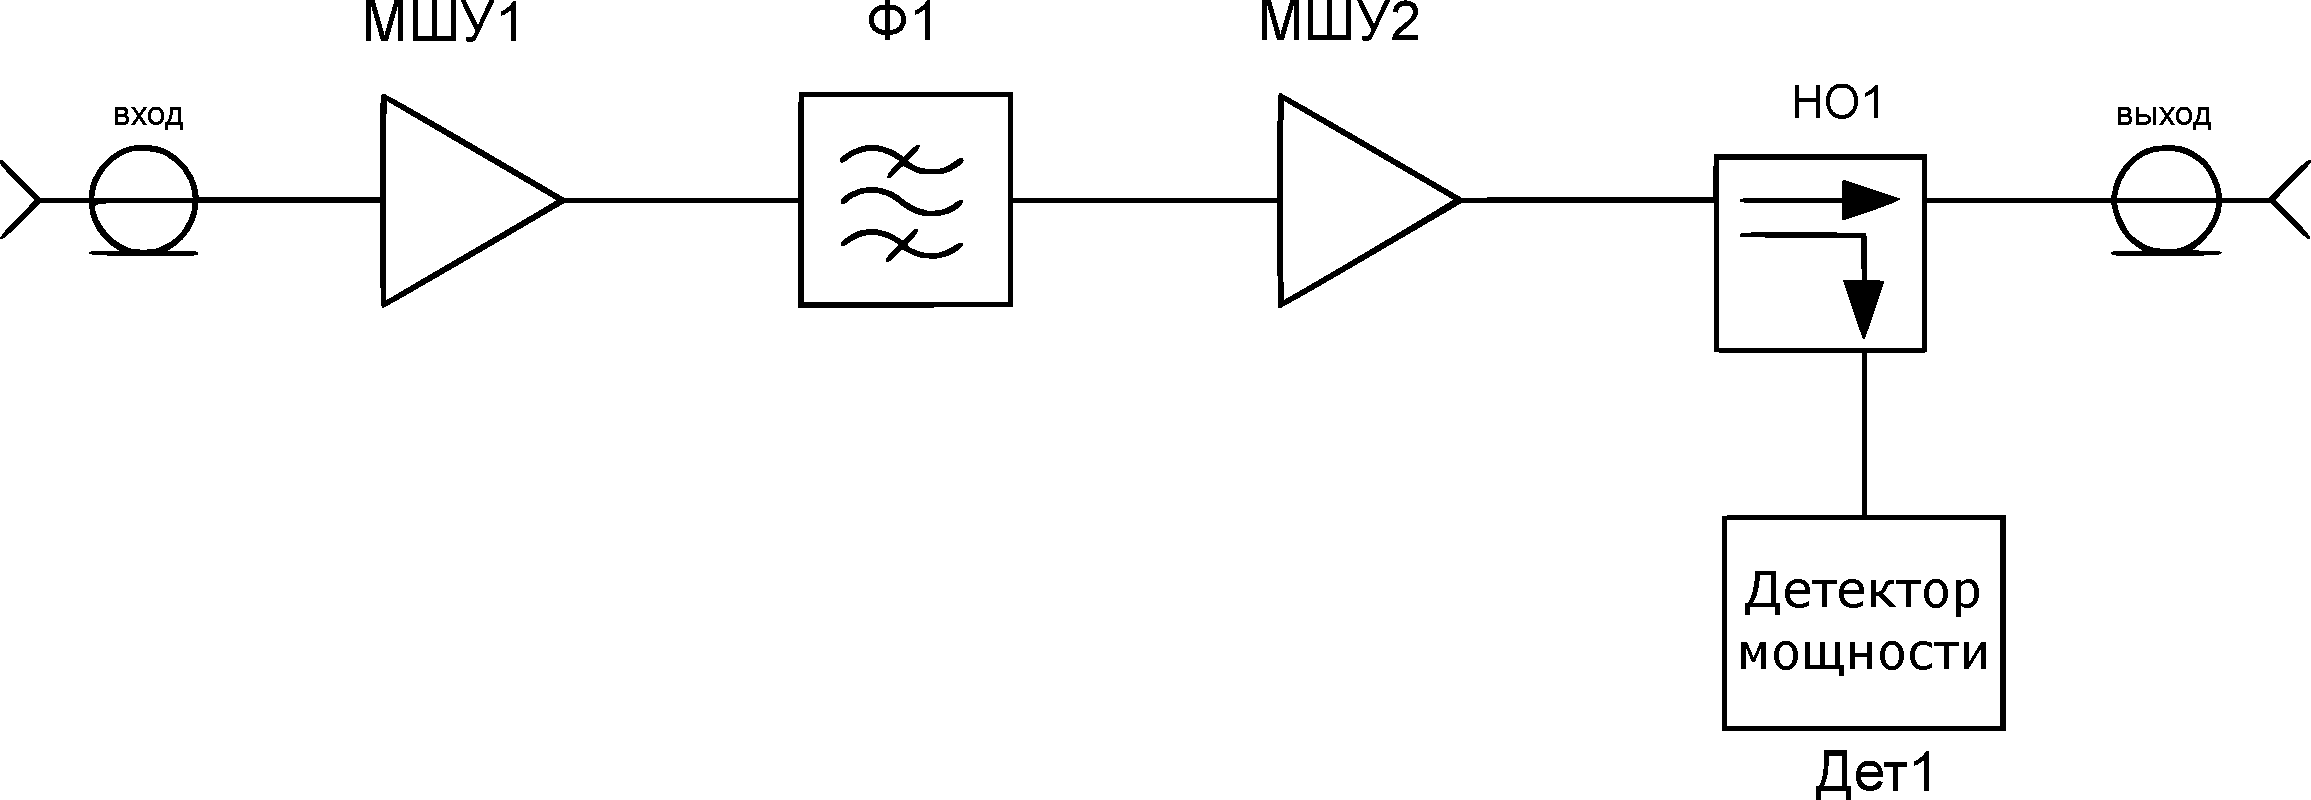
\includegraphics[width=0.8\textwidth,height=0.4\textheight,keepaspectratio]{MainStrSch.pdf}
				\vspace*{0.05\textheight}
			\end{figure}
			
			
			Приемная ячейка усиления и фильтрации с детектированием мощности
		\end{center}
		
		
	\end{frame}
	
\subsection{Ожидаемые характеристики}
	
	\begin{frame}
		\frametitle{\insertsection}
		\framesubtitle{\insertsubsection}
		\begin{center}
			\begin{figure}
				\centering
			%	\vspace{0.1\textheight}
				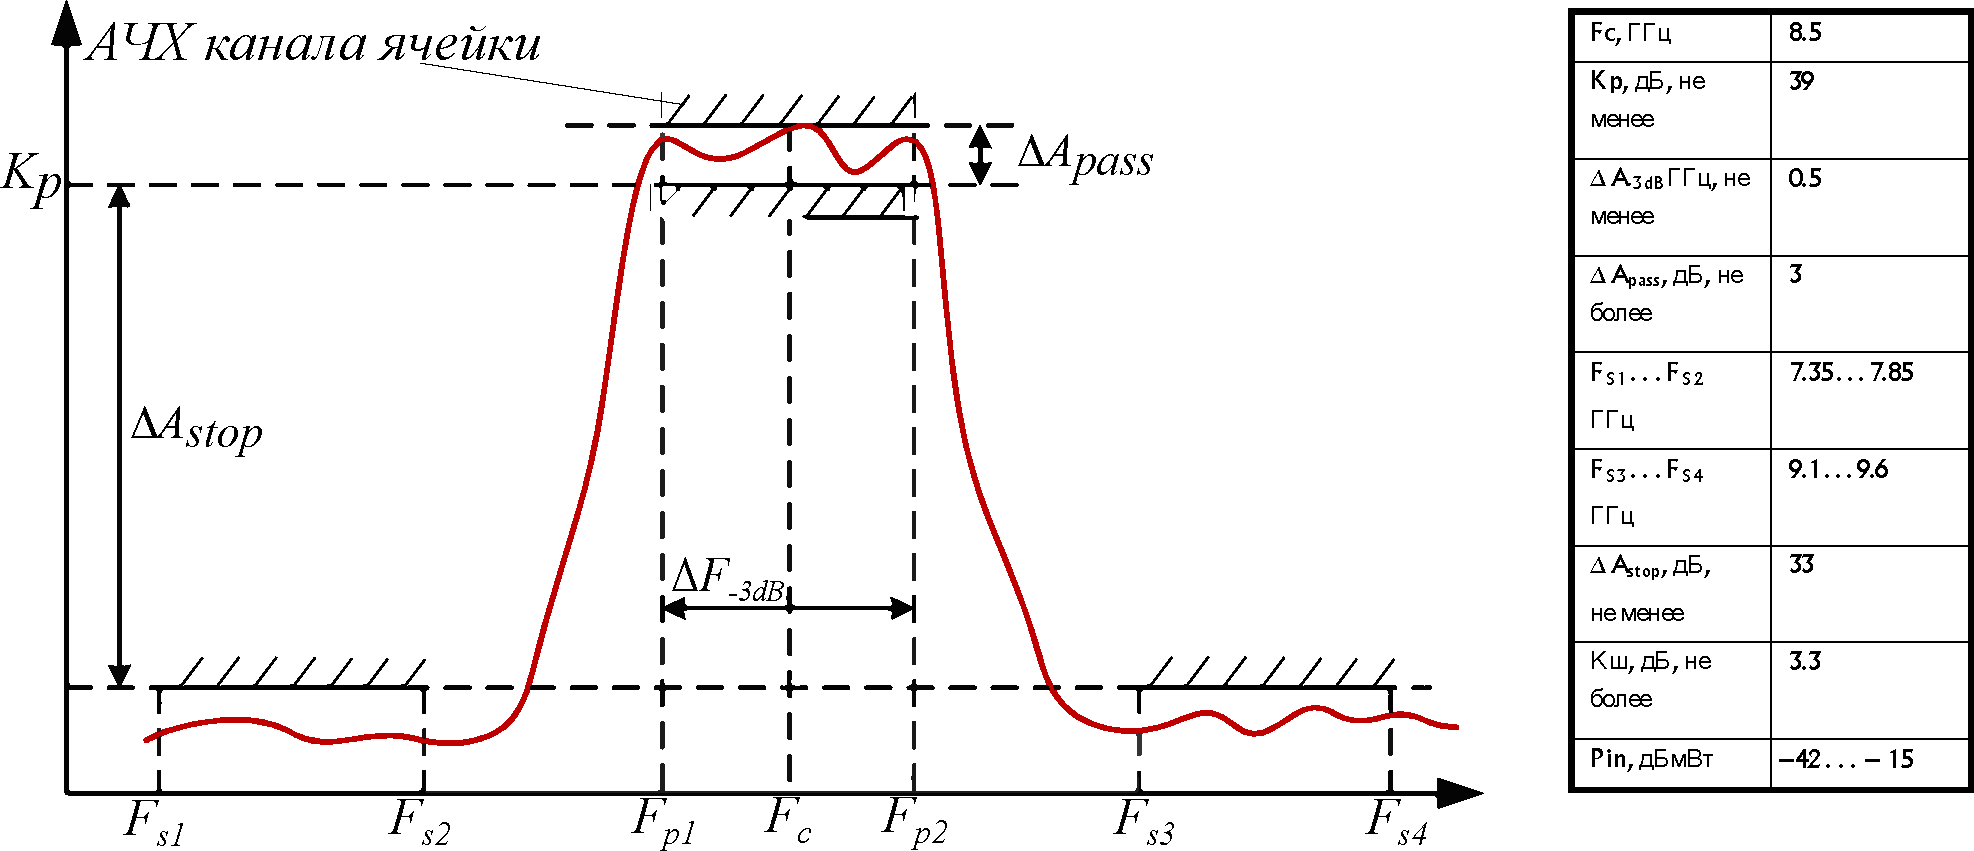
\includegraphics[width=\textwidth,height=0.9\textheight,keepaspectratio]{TZ+table.pdf}
			\end{figure}
		\end{center}
	\end{frame}

\section{Выбор ВЧ-элементной базы}
\subsection{Выбор МШУ}
	\begin{frame}[shrink=30]
			\frametitle{\insertsection}
			\framesubtitle{\insertsubsection}
			\begin{center}
				\begin{figure}
					\begin{subfigure}[t]{0.5\textwidth}
						\vspace{-1\textheight}%
						\begin{subfigure}[t]{\textwidth}
							\begin{center}
								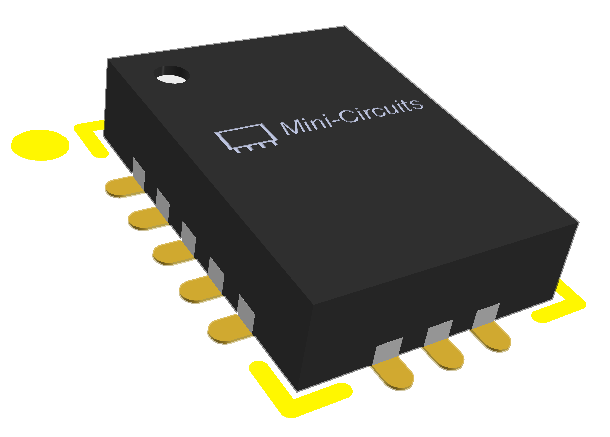
\includegraphics[width=\textwidth, height = 0.6\textheight, keepaspectratio]{LNA_3D_View.png}
								\vspace*{0.05\textheight} 
							\end{center}
						\end{subfigure}
					
						\begin{subfigure}[b]{\textwidth}
							\begin{center}
								\begin{tabular}{|c|c|c|c|}
									\hline
									F & Kу & NF & IP3 \\
									\hline
									6 --- 18 ГГц & 26 дБ & 1.2 дБ & 30 дБм \\
									\hline
								\end{tabular}
							\end{center}
						\end{subfigure}
					\end{subfigure}%
					%
					\begin{subfigure}[b]{0.5\textwidth}
							\begin{subfigure}[t]{\textwidth}
								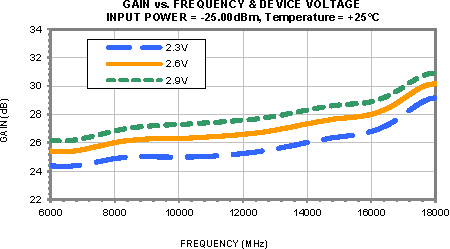
\includegraphics[width=\textwidth]{PMA-GvsFvsV.pdf}
							\end{subfigure}
						
							\begin{subfigure}[b]{\textwidth}
								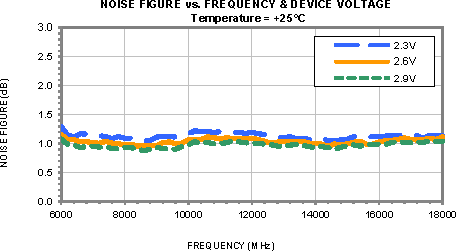
\includegraphics[width=\textwidth]{PMA-NFvsFvsV.pdf}
							\end{subfigure}
					\end{subfigure}
				\end{figure}
			\end{center}
	\end{frame}

\subsection{Выбор детектора мощности}\label{susec:PD_choosing}

	\begin{frame}
		\frametitle{\insertsection}
		\framesubtitle{\insertsubsection}
		\begin{center}
			\begin{figure}
				\begin{subfigure}{0.5\textwidth}
					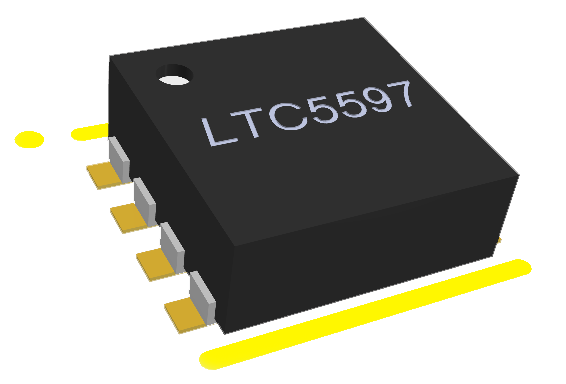
\includegraphics[width=0.9\textwidth,height =\textheight, keepaspectratio]{PD_3D_View.png}
				\end{subfigure}%
				%
				\begin{subfigure}{0.5\textwidth}
					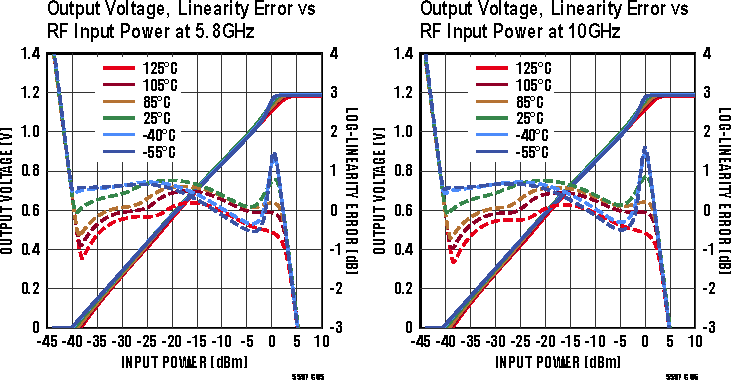
\includegraphics[width=0.9\textwidth,height =\textheight, keepaspectratio, trim={0cm 0cm 6.1cm 0.8cm}, clip]{LTC-power-limits.pdf}
				\end{subfigure}
			\end{figure}
		Зависимость выходного напряжения и ошибки от входной мощности в рабочей полосе.
		\end{center}
		
			
	\end{frame}

\subsection{Выбор ВЧ-подложки}

	\begin{frame}
		\frametitle{\insertsection}
		\framesubtitle{\insertsubsection}
		
		\begin{center}
			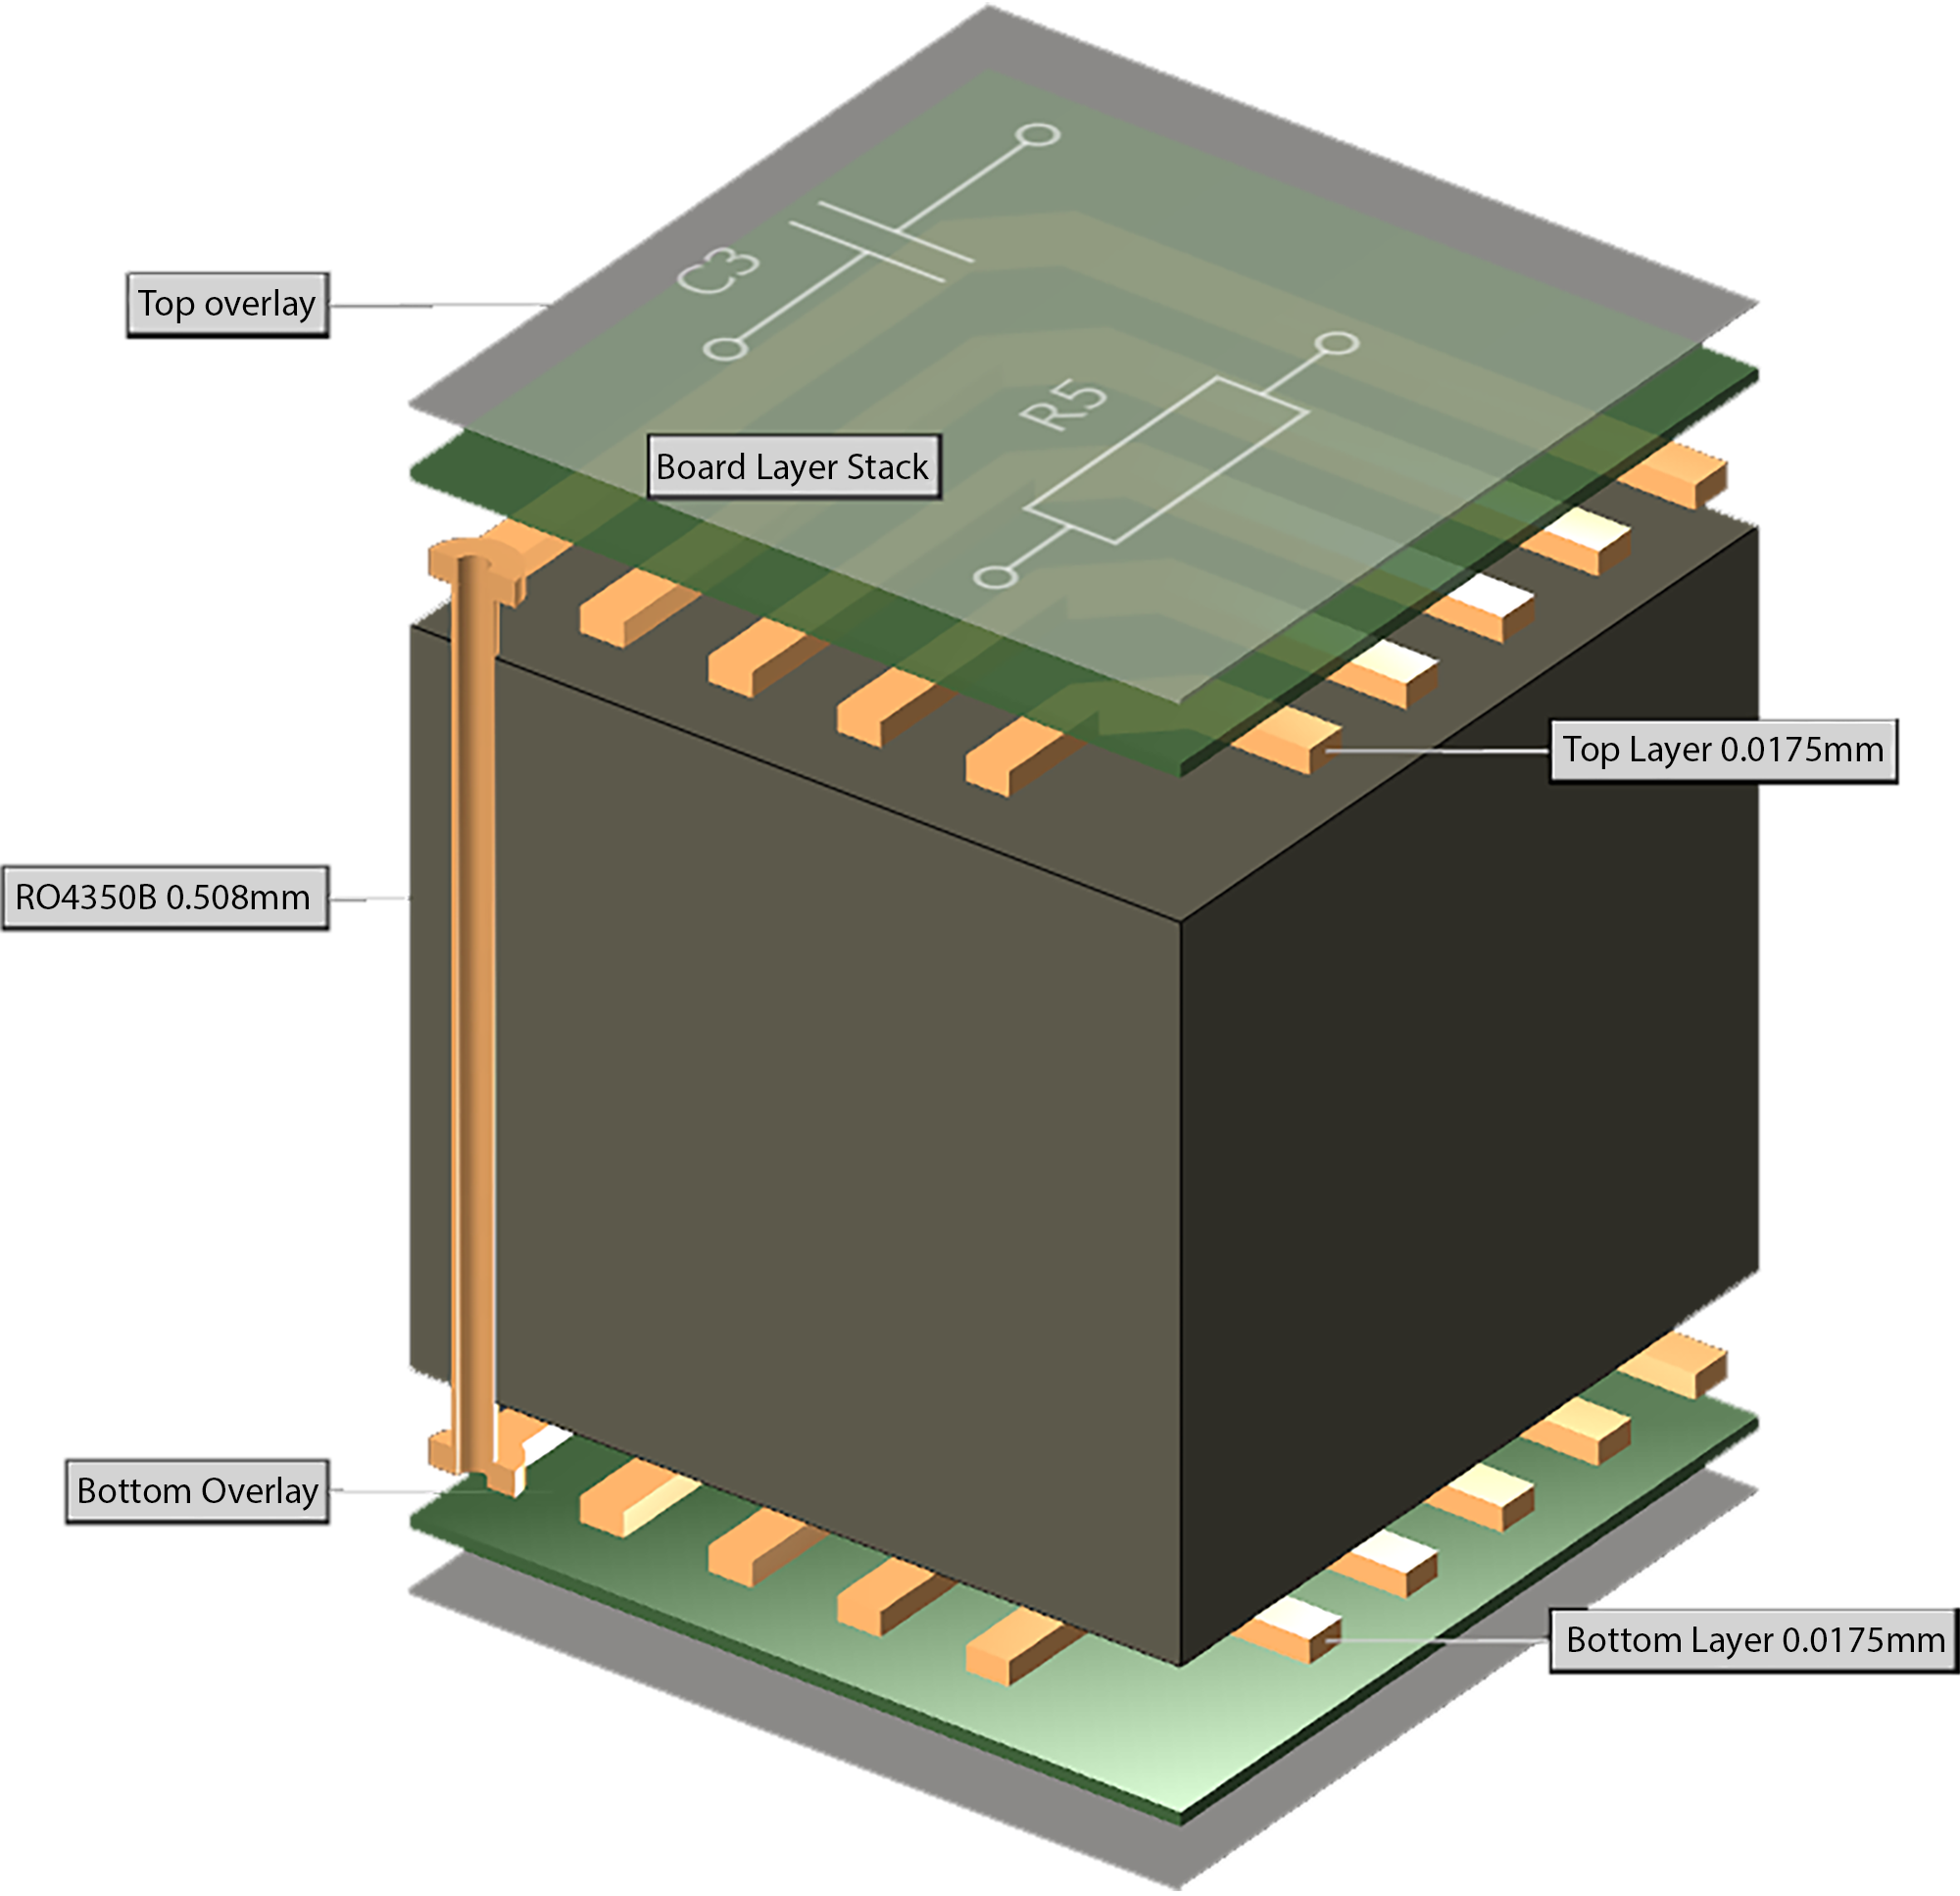
\includegraphics[width=0.9\textwidth, height=0.8\textheight, keepaspectratio]{LayerStack3D.png}
		\end{center}
		
	\end{frame}
	
\section{Выбор дополнительной элементной базы}
\subsection{Выбор микроконтроллера и стабилизаторов напряжения}

	\begin{frame}[shrink=20]
		\frametitle{\insertsection}
		\framesubtitle{\insertsubsection}
		\begin{center}
			\begin{figure}
				\begin{subfigure}{0.5\textwidth}
					\begin{subfigure}[t]{0.95\textwidth}
						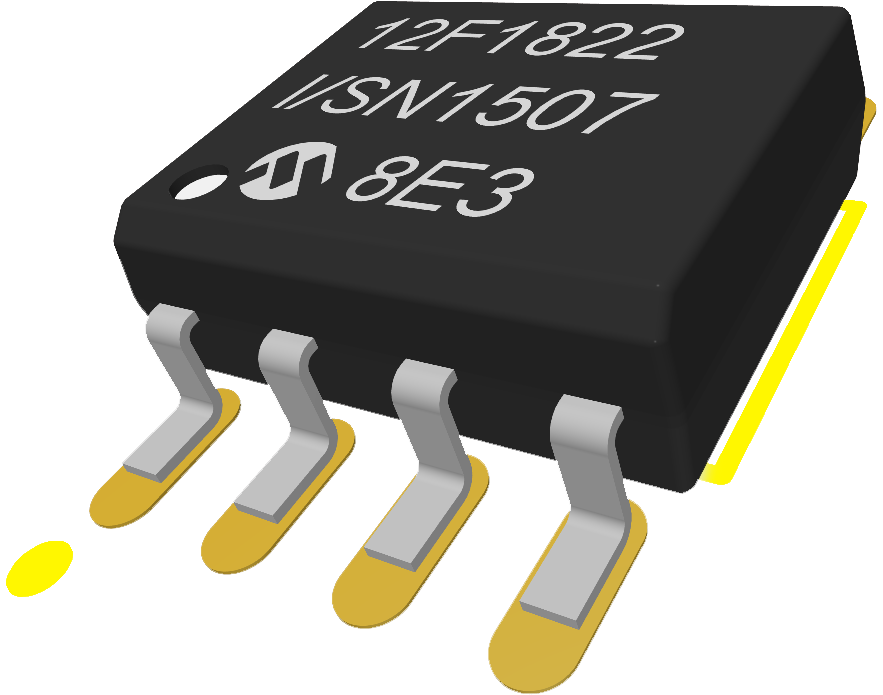
\includegraphics[height=0.4\paperheight, keepaspectratio]{MC_3D_View.png}
					\end{subfigure}
					
					\begin{subfigure}[b]{0.95\textwidth}
						\begin{itemize}
							\item 3.3~В рабочее напряжение;
							\item 10-битный АЦП с настраиваемым диапазоном;
							\item Поддержка USART, SPI и I2C.
						\end{itemize}
					\end{subfigure}
				\end{subfigure}%
				%
				\begin{subfigure}{0.5\textwidth}
					\begin{subfigure}[t]{0.95\textwidth}
						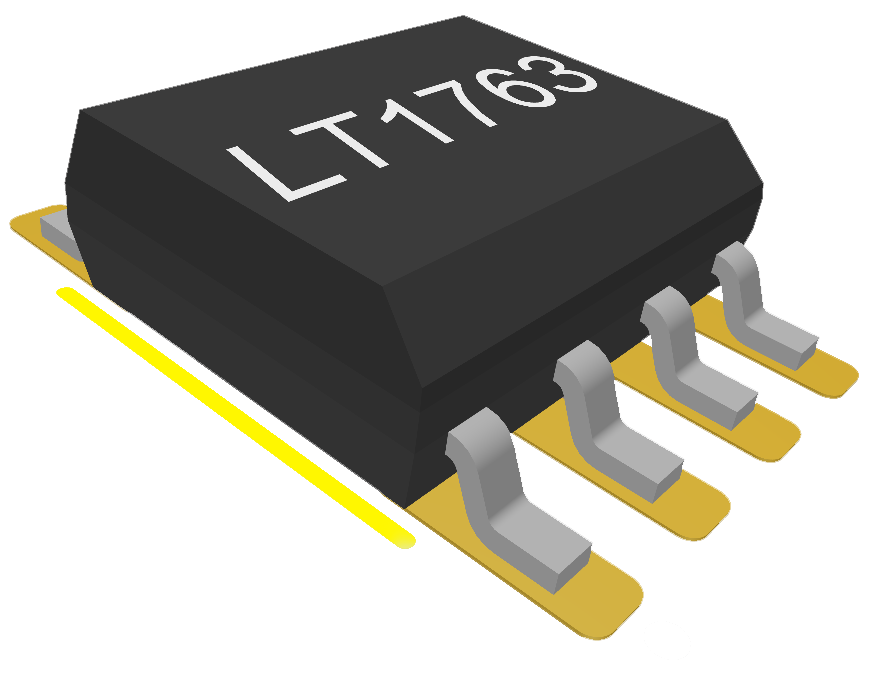
\includegraphics[height=0.45\paperheight, keepaspectratio]{PM_3D_View.png}
					\end{subfigure}
					
					\begin{subfigure}[b]{0.95\textwidth}
						\begin{itemize}
							\item Входное напряжение 2.2 \textdiv\  20~В 
							\item Фиксированные выходные напряжения: 1.5, 1.8, 2.5, 3, 3.3, 5~В
							\item Выходной ток до 0.5~А
						\end{itemize}
					\end{subfigure}
				\end{subfigure}
			\end{figure}
		
		\end{center}
	\end{frame}

\section{Моделирование в среде Keysight ADS}
\subsection{Согласование компонентов}
	\begin{frame}
		\frametitle{\insertsection}
		\framesubtitle{\insertsubsection}
		\centering
		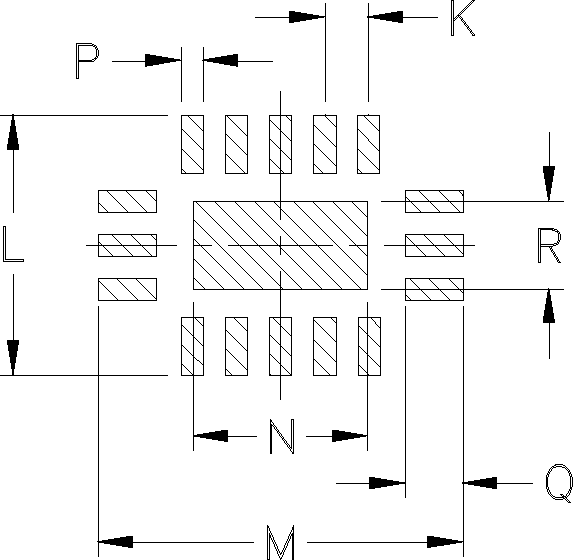
\includegraphics[width=\textwidth, height=0.5\textheight, keepaspectratio]{PMA-Place.pdf}
		
		\vfill
		Посадочное место МШУ
		
	\end{frame}

	\begin{frame}
		\frametitle{\insertsection}
		\framesubtitle{\insertsubsection}
		\centering
		\hspace*{-0.075\textwidth}%
		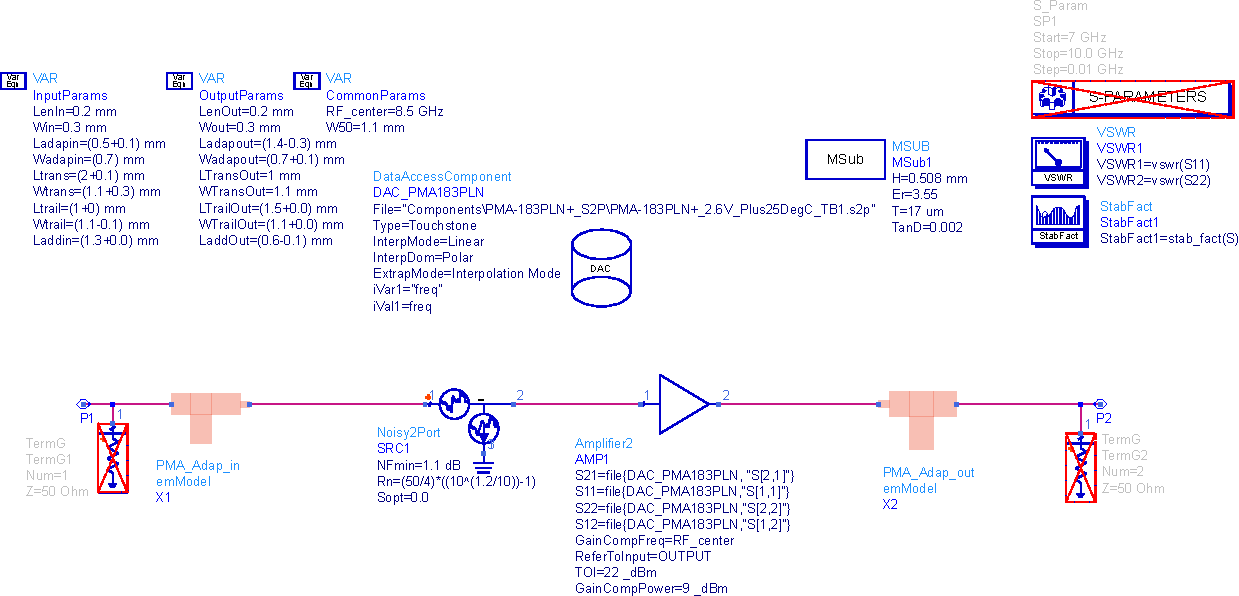
\includegraphics[width=1.15\textwidth, height=0.8\textheight, keepaspectratio]{LNA_Sch.pdf}
		
		\vfill 
		Схема включения МШУ
	\end{frame}


	\begin{frame}
		\frametitle{\insertsection}
		\framesubtitle{\insertsubsection}
		\centering
		%\hspace*{-0.05\textwidth}%
		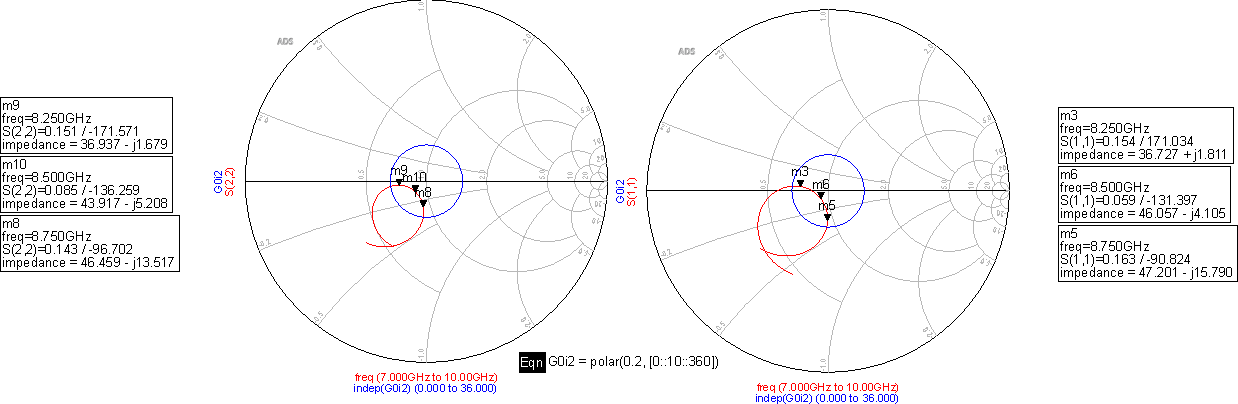
\includegraphics[width=0.9\paperwidth, height=\textheight, keepaspectratio]{LNA_Response_Z.pdf}
		
	\end{frame}
	
	\begin{frame}
		\frametitle{\insertsection}
		\framesubtitle{\insertsubsection}
		\centering
		%\hspace*{-0.075\textwidth}%
		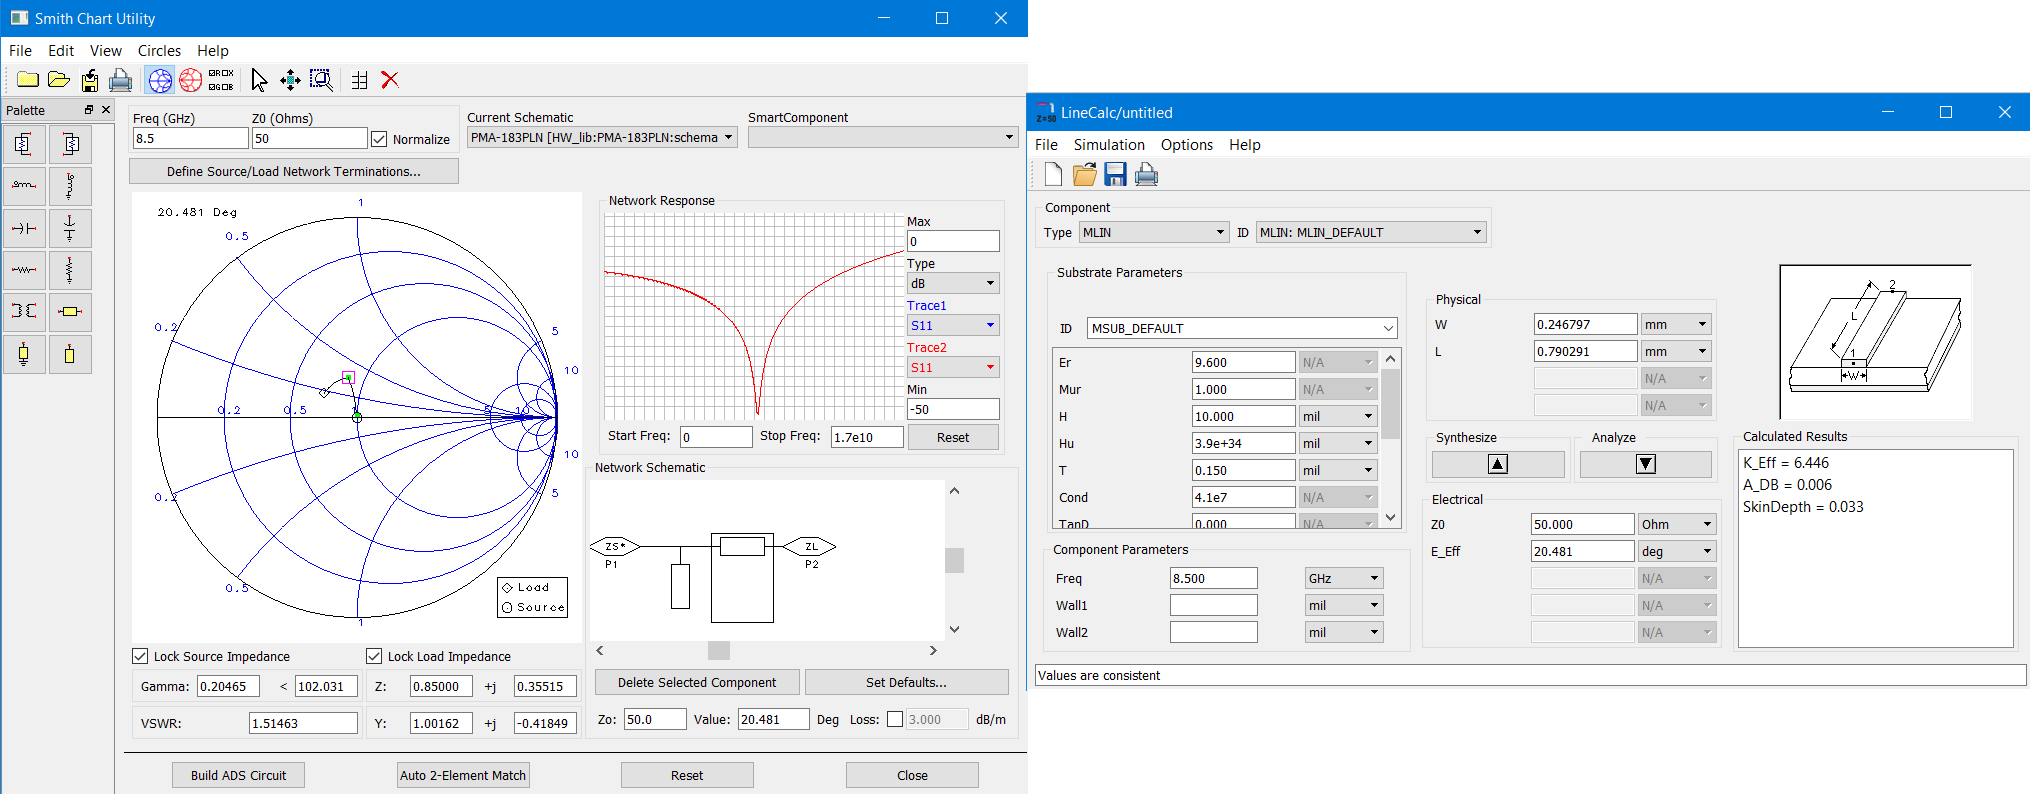
\includegraphics[width=0.9\paperwidth, height=\textheight, keepaspectratio]{Utilities.png}
		
	\end{frame}

	\begin{frame}
		\frametitle{\insertsection}
		\framesubtitle{\insertsubsection}
		\begin{center}
			\begin{figure}
				\begin{subfigure}{0.45\paperwidth}
					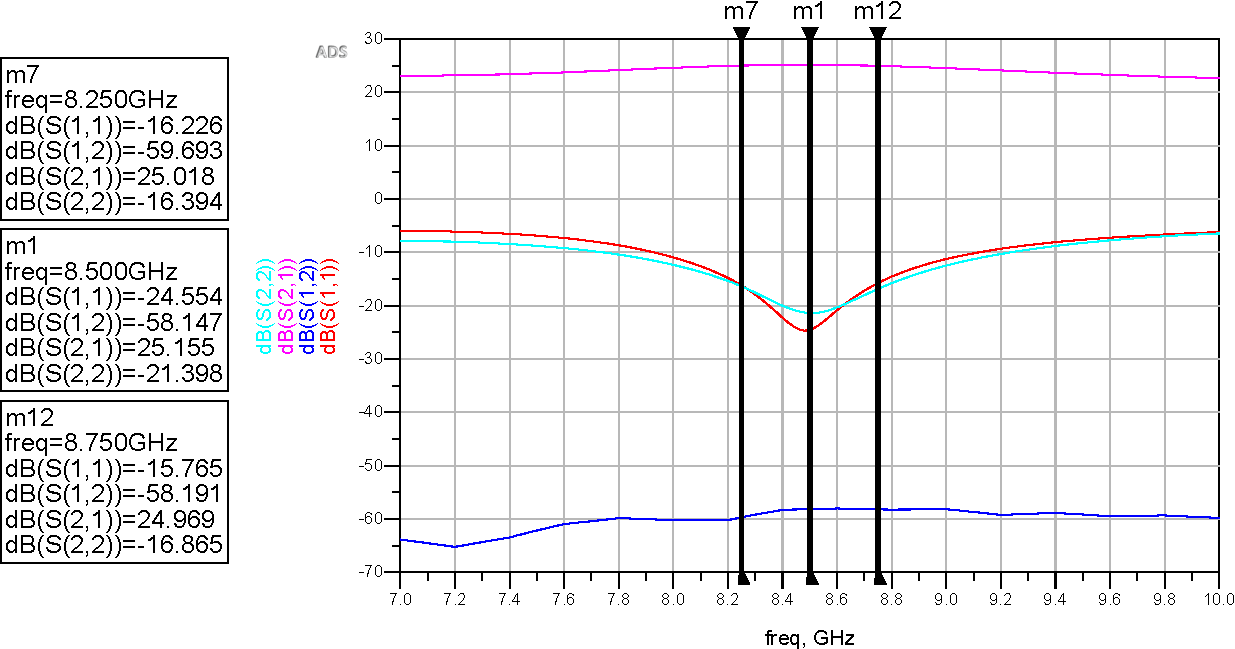
\includegraphics[width=\textwidth,keepaspectratio]{LNA_Response.pdf}%
				\end{subfigure}%
				\begin{subfigure}{0.45\paperwidth}
					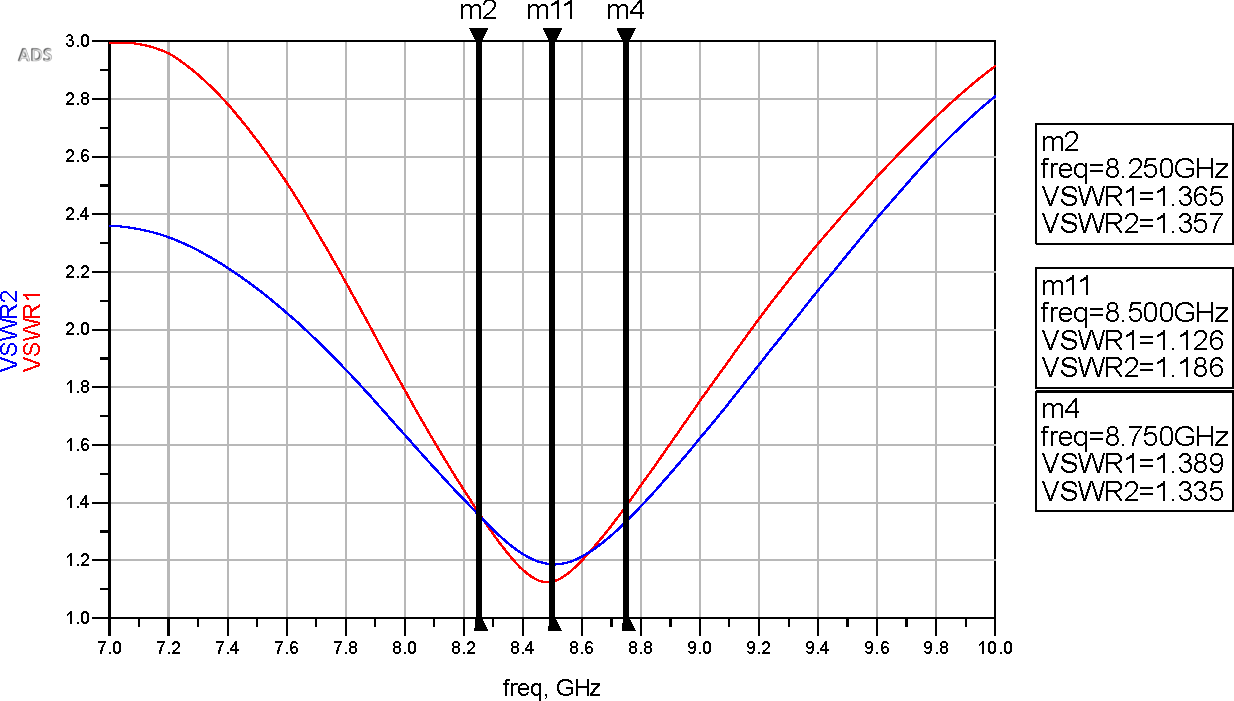
\includegraphics[width=\textwidth,keepaspectratio]{LNA_VSWR.pdf}
				\end{subfigure}
			\end{figure}
		\end{center}
	\end{frame}
	
	\begin{frame}
		\frametitle{\insertsection}
		\framesubtitle{\insertsubsection}
		\centering
		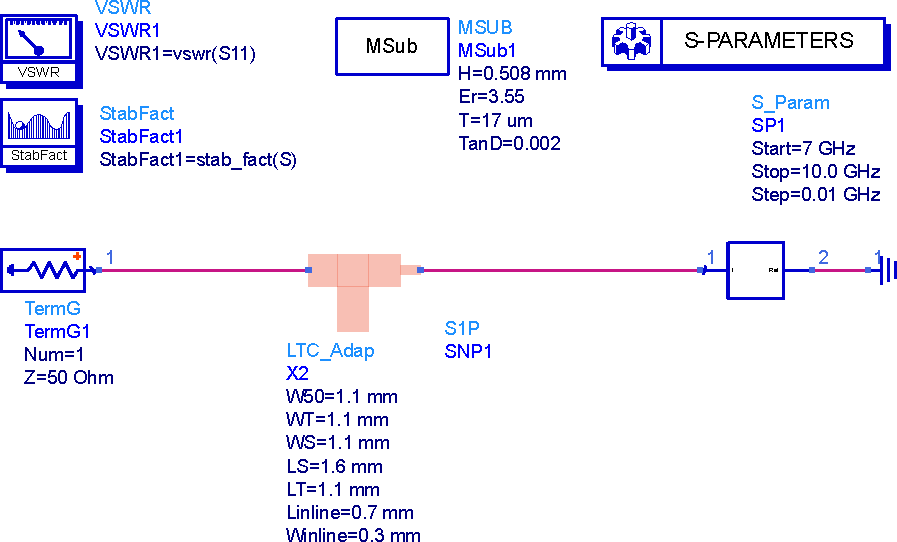
\includegraphics[width=\textwidth, height=0.6\textheight, keepaspectratio]{LTC_Sch.pdf}
		
	\end{frame}

\subsection{Проектирование фильтра}

	\begin{frame}
		\frametitle{\insertsection}
		\framesubtitle{\insertsubsection}
		\centering
		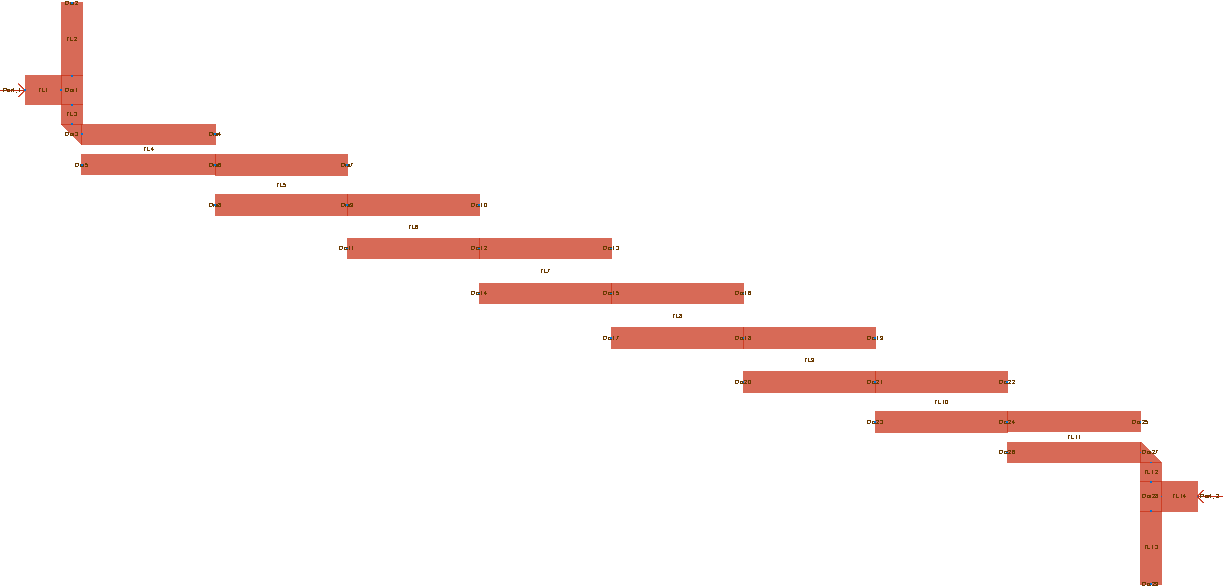
\includegraphics[width=\textwidth, height=0.6\textheight, keepaspectratio]{FilterLayout.pdf}
	\end{frame}

	\begin{frame}
		\frametitle{\insertsection}
		\framesubtitle{\insertsubsection}
		\centering
		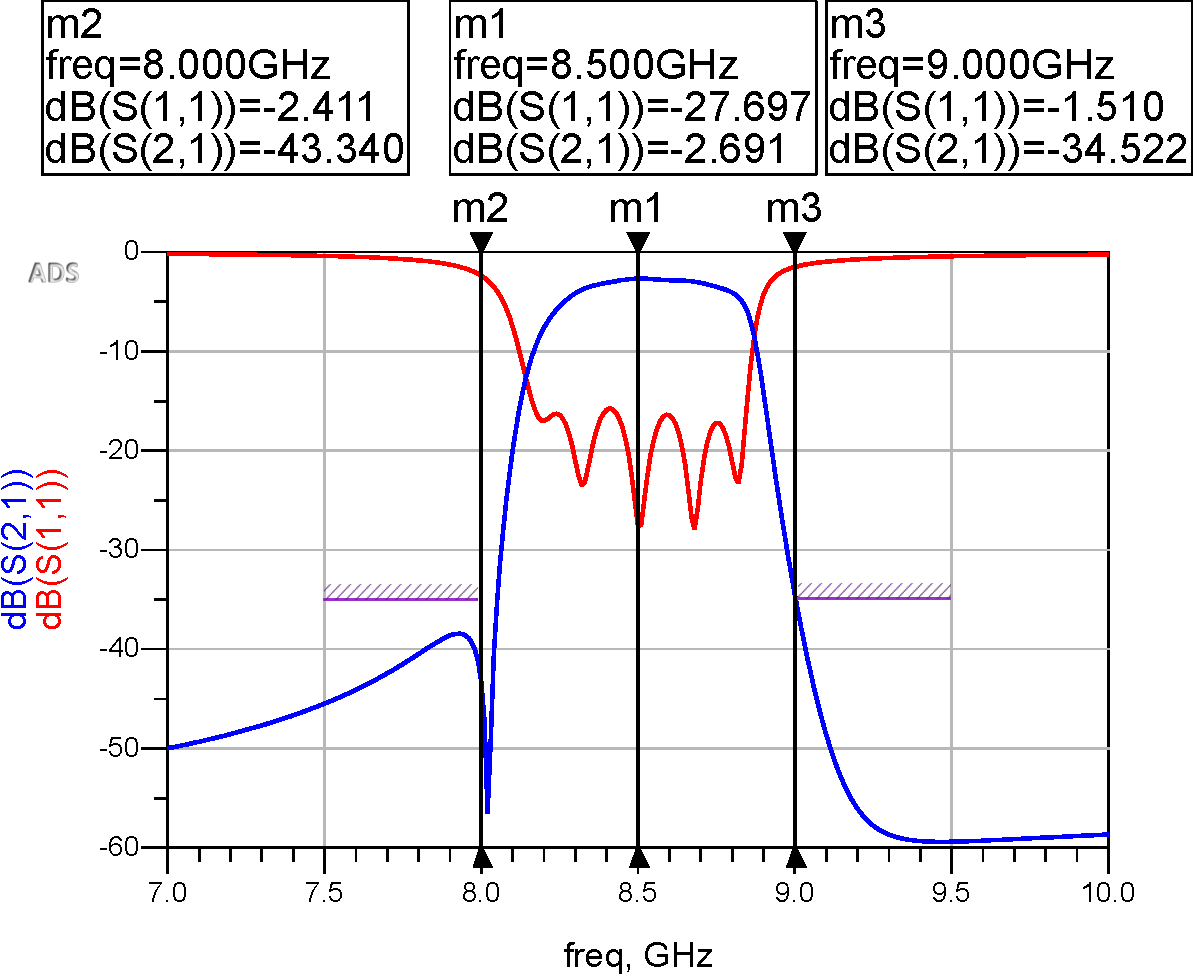
\includegraphics[width=\textwidth, height=0.6\textheight, keepaspectratio]{FilterResponse.pdf}
		
	\end{frame}

\subsection{Проектирование ответвителя}

	\begin{frame}
		\frametitle{\insertsection}
		\framesubtitle{\insertsubsection}
		\centering
		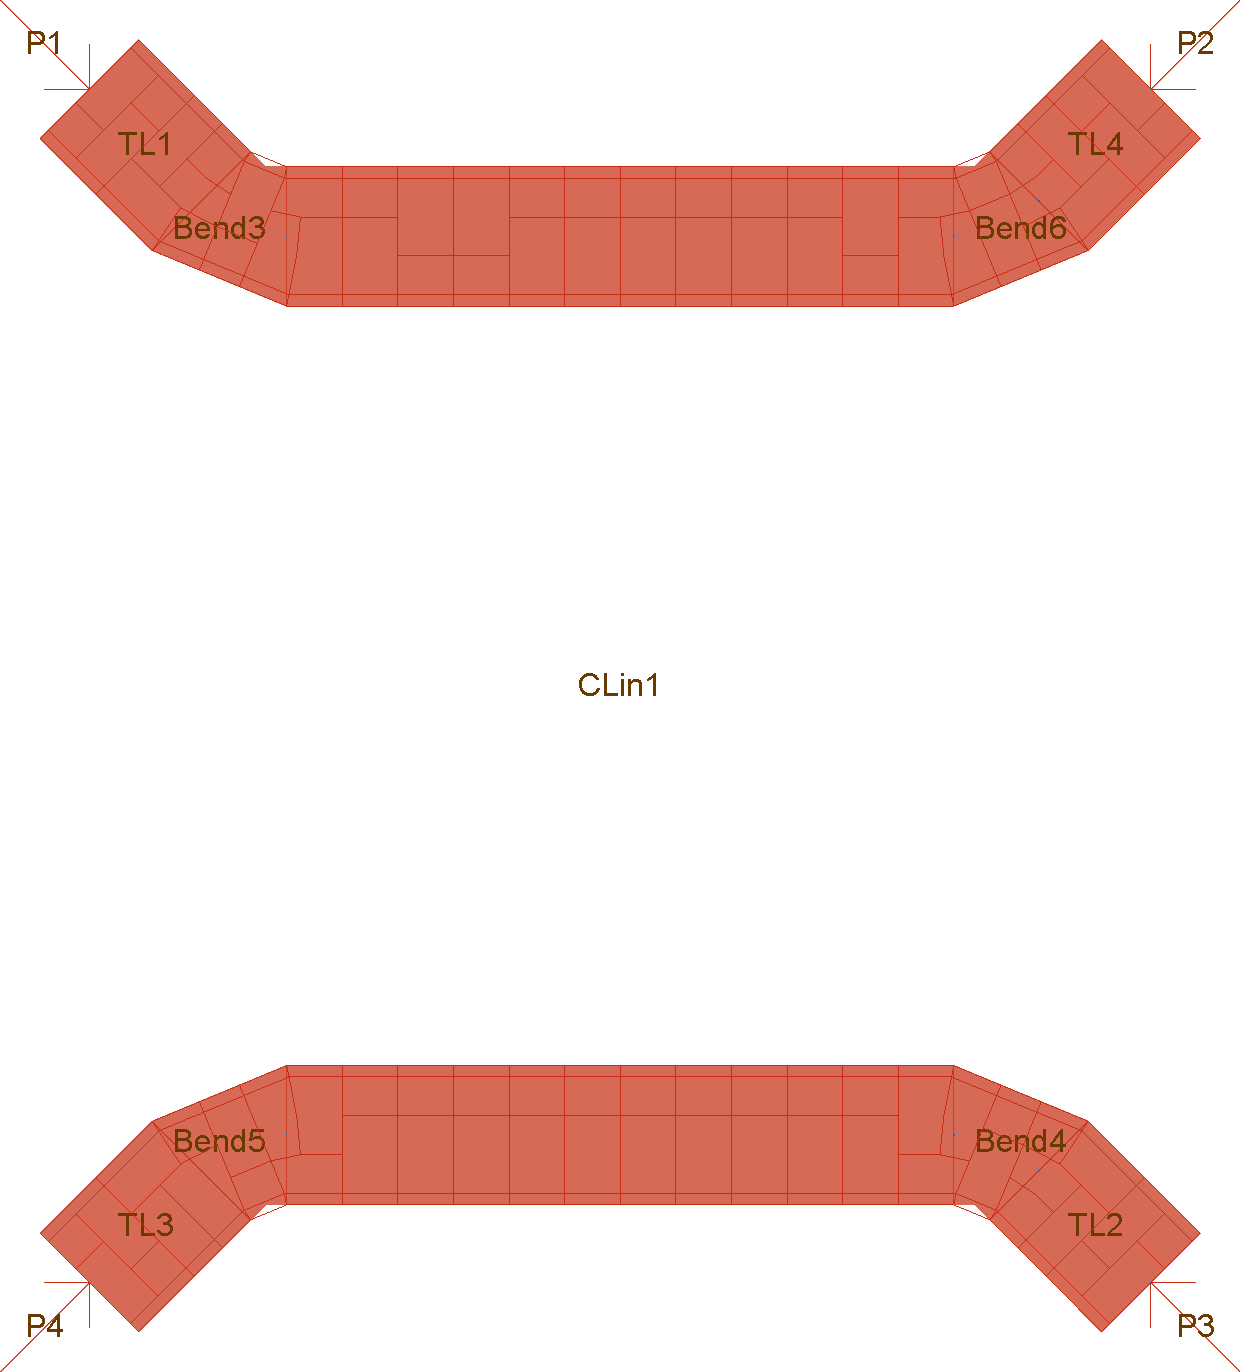
\includegraphics[width=\textwidth, height=0.6\textheight, keepaspectratio]{CLC_Layout.pdf}
	\end{frame}
	
	\begin{frame}
		\frametitle{\insertsection}
		\framesubtitle{\insertsubsection}
		\centering
		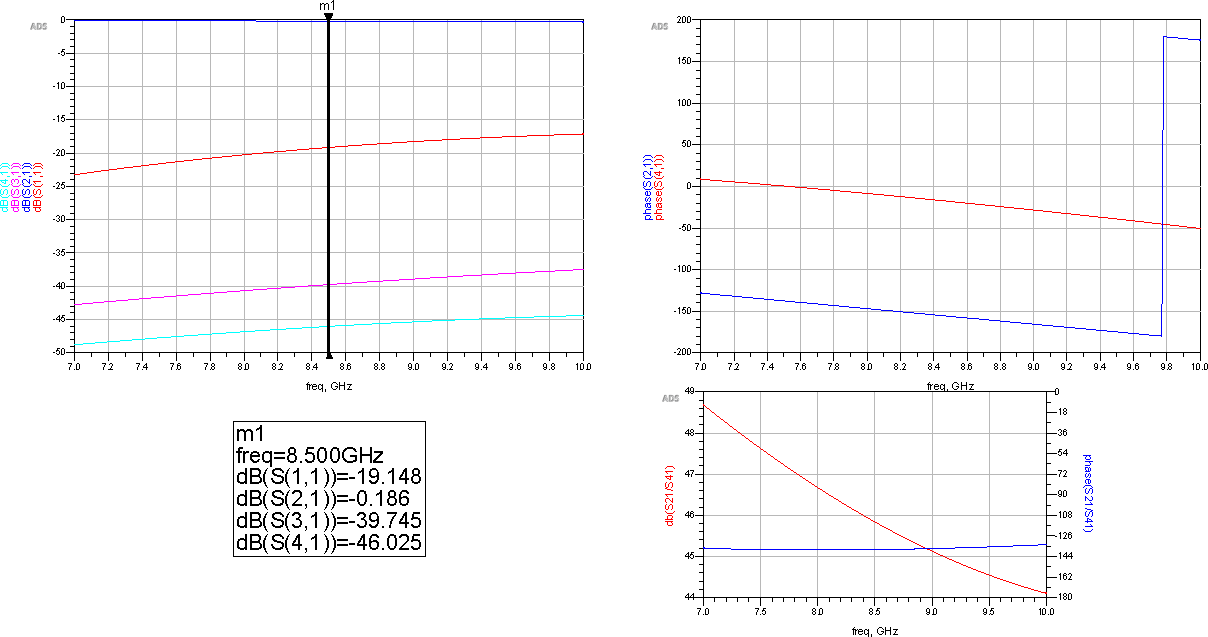
\includegraphics[width=\textwidth, height=0.6\textheight, keepaspectratio]{CLC_Response.pdf}
		
	\end{frame}

\subsection{Системное моделирование}

	\begin{frame}
		\frametitle{\insertsection}
		\framesubtitle{\insertsubsection}
		\centering
		%\hspace*{-0.075\textwidth}%
		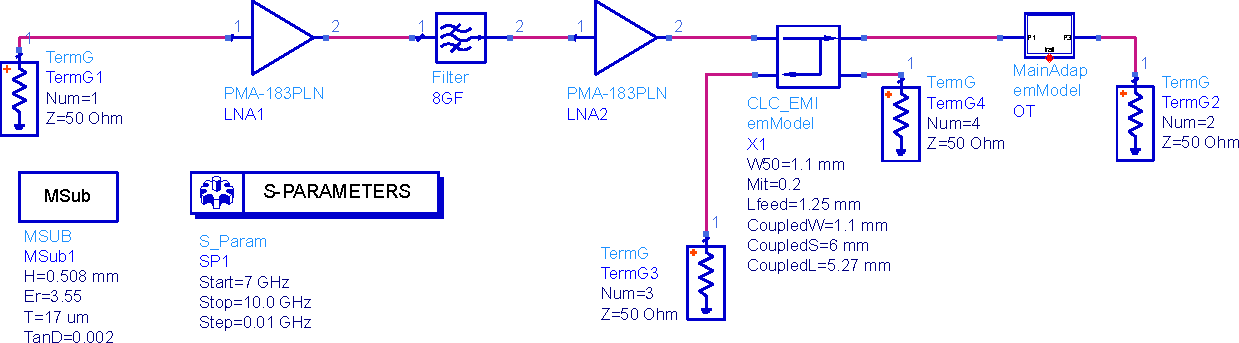
\includegraphics[width=0.9\paperwidth, height=0.95\textheight, keepaspectratio]{SystemSch.pdf}
		
	\end{frame}
	
	\begin{frame}
		\frametitle{\insertsection}
		\framesubtitle{\insertsubsection}
		\centering
		%\hspace*{-0.075\textwidth}%
		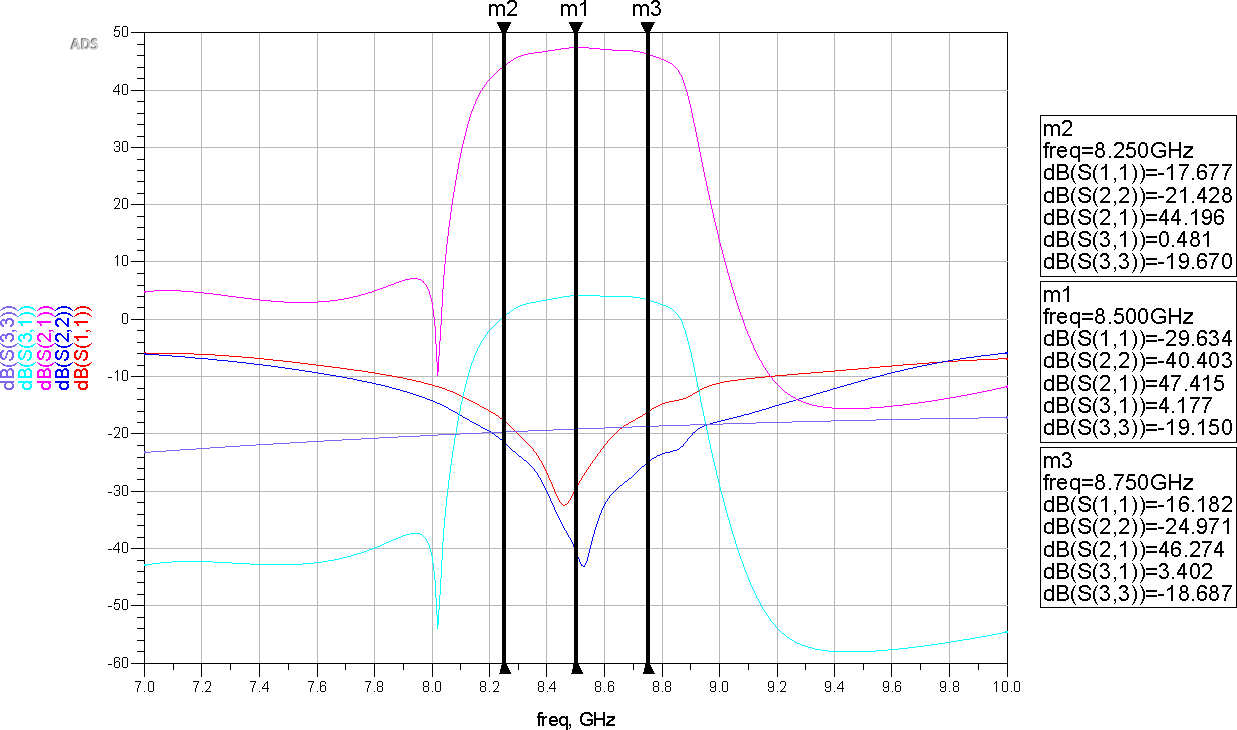
\includegraphics[width=0.9\paperwidth, height=0.85\textheight, keepaspectratio]{SystemResponse.pdf}
		
	\end{frame}

\subsection{Шумовая характеристика}
	
	\begin{frame}
		\frametitle{\insertsection}
		\framesubtitle{\insertsubsection}
		\centering
		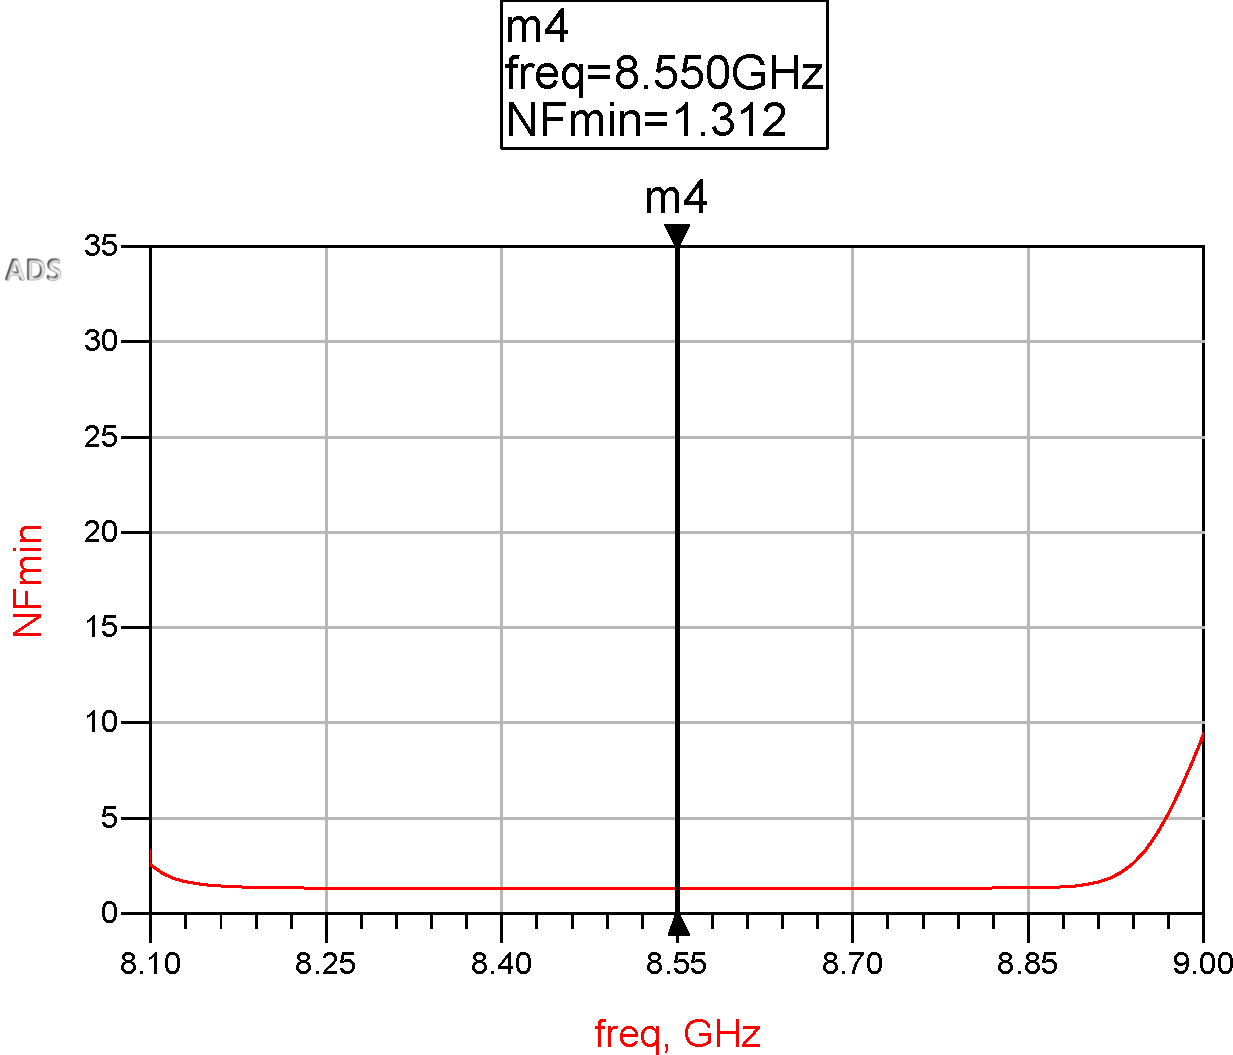
\includegraphics[width=1.15\textwidth, height=0.6\textheight, keepaspectratio]{SystemNF.pdf}
		
	\end{frame}

\section{Проектирование печатной платы}
\subsection{Э3}

	\begin{frame}
		\frametitle{\insertsection}
		\framesubtitle{\insertsubsection}
		\centering
		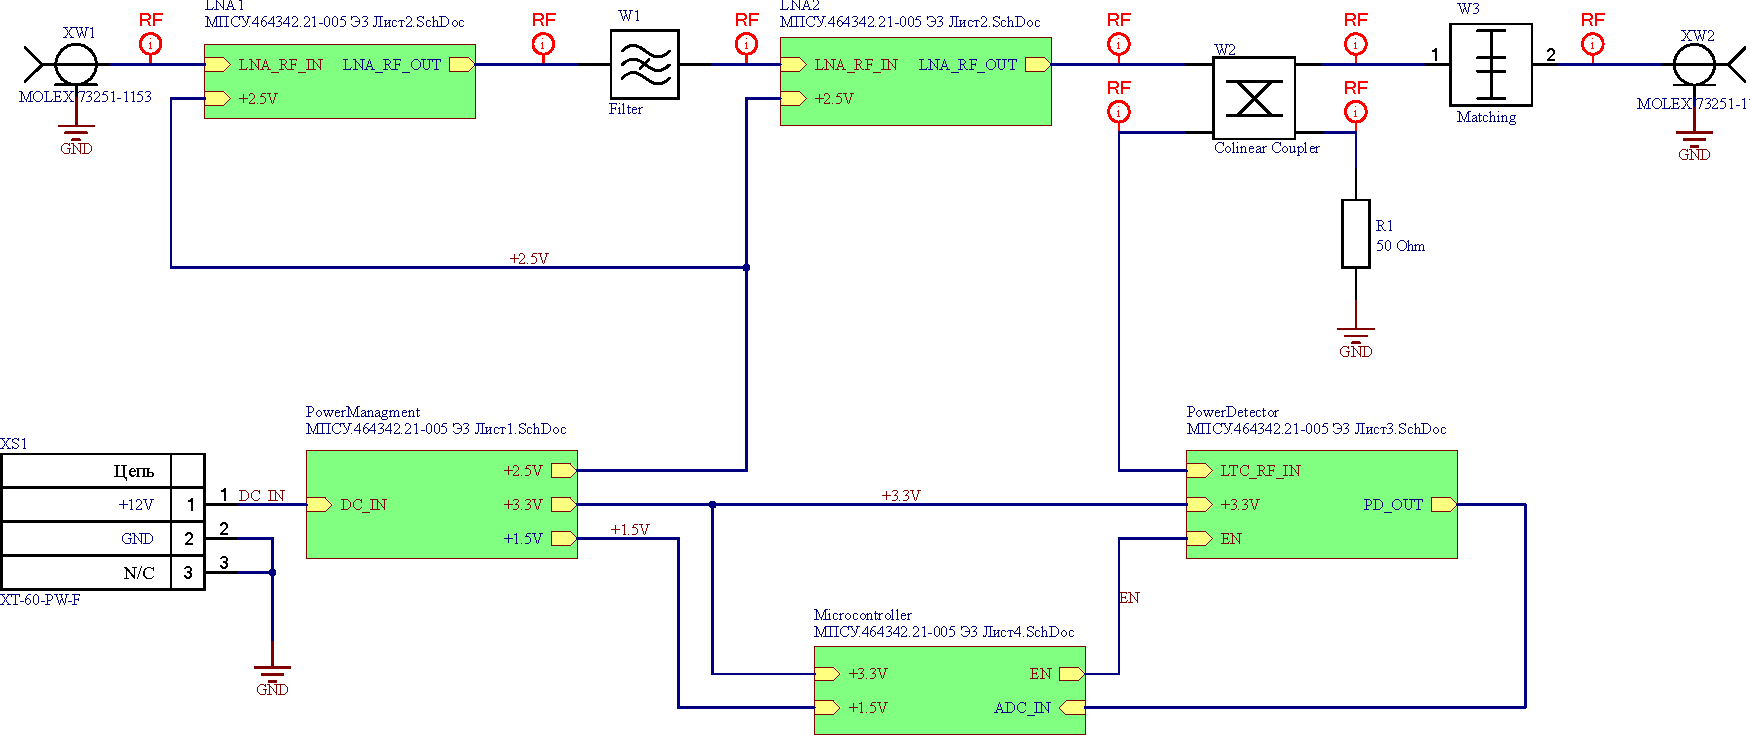
\includegraphics[width=\textwidth, height=0.6\textheight, keepaspectratio]{Main_SchDoc.pdf}		
	\end{frame}

\subsection{МШУ}
	
	\begin{frame}
		\frametitle{\insertsection}
		\framesubtitle{\insertsubsection}
		\centering
		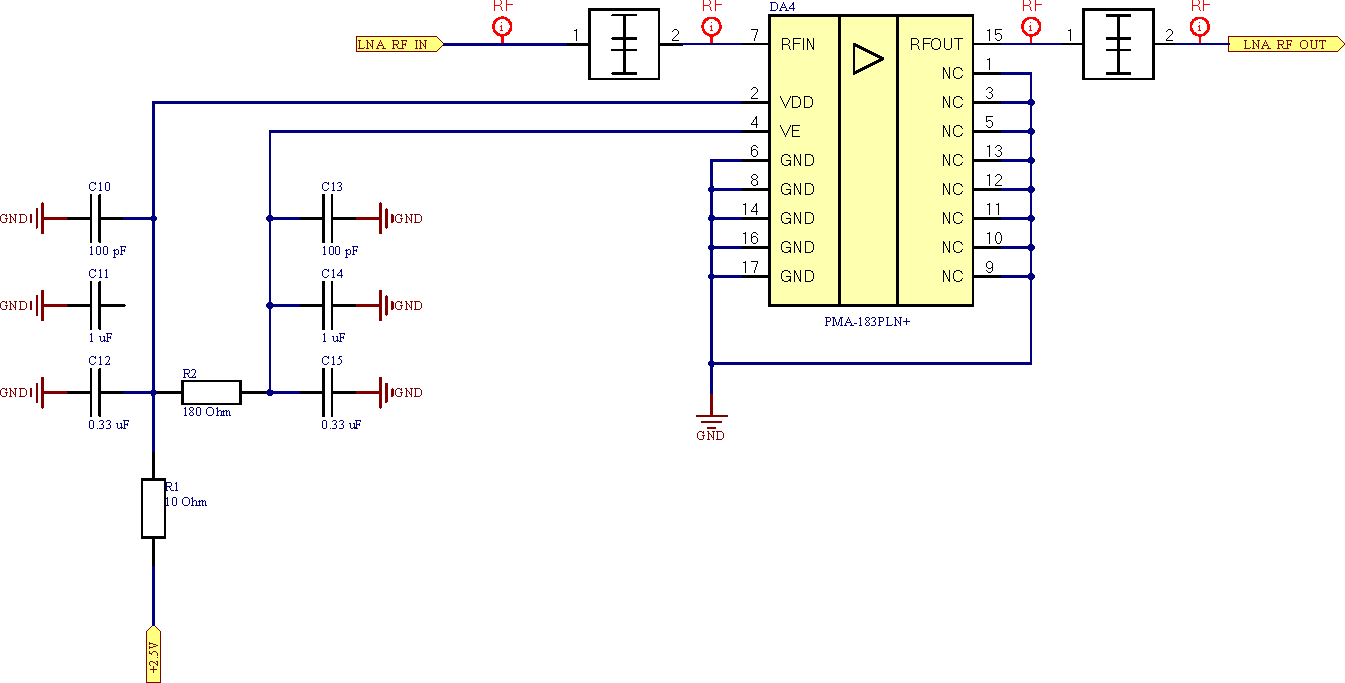
\includegraphics[width=\textwidth, height=0.6\textheight, keepaspectratio]{LNA_SchDoc.pdf}
	\end{frame}

\subsection{Детектор мощности}
	
	\begin{frame}
		\frametitle{\insertsection}
		\framesubtitle{\insertsubsection}
		\centering
		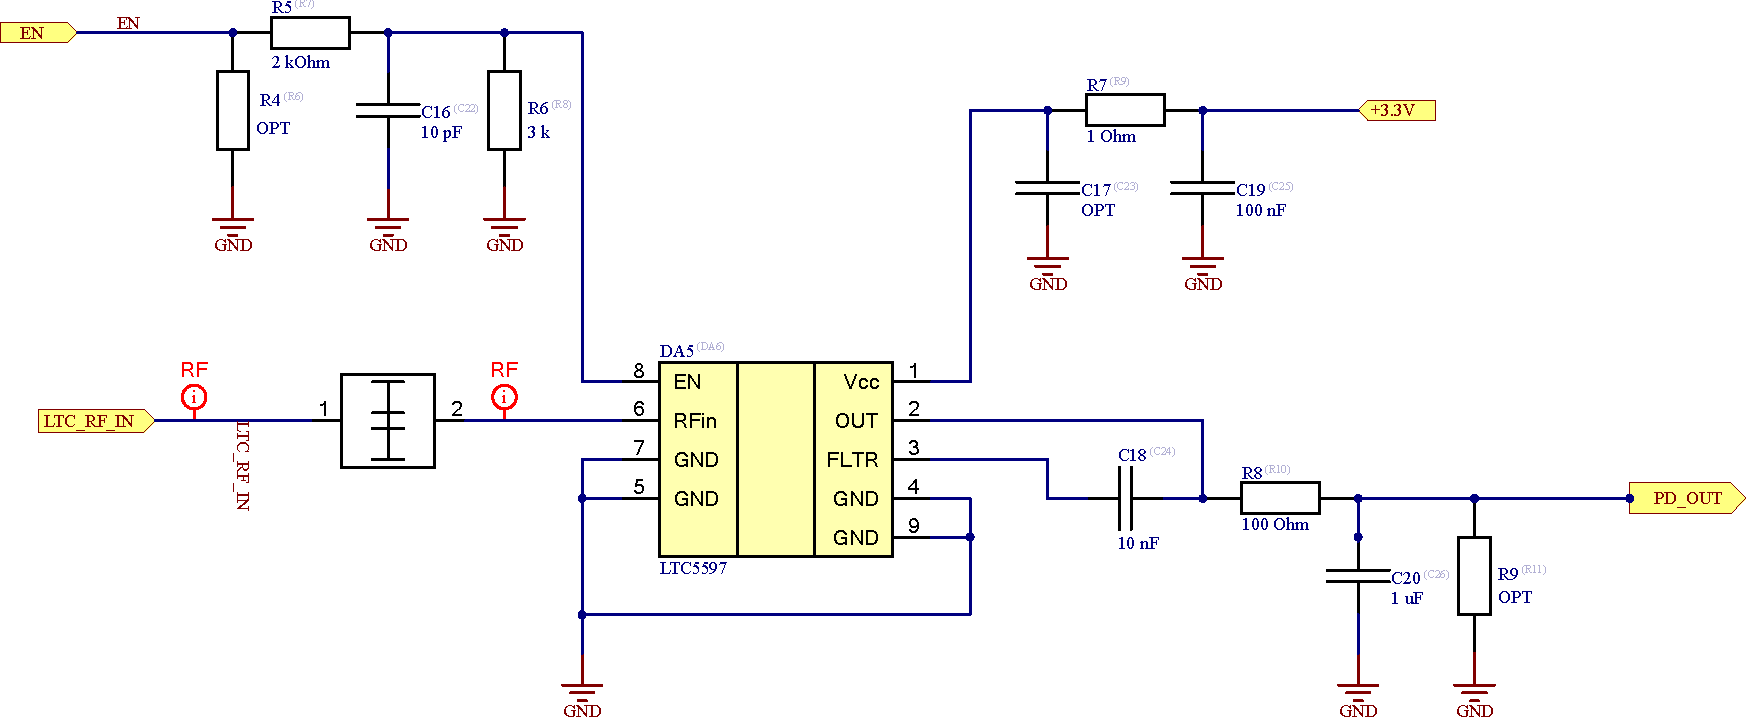
\includegraphics[width=\textwidth, height=0.6\textheight, keepaspectratio]{PD_SchDoc.pdf}	
		
		\vfill
		\hyperlink{susec:PD_choosing}{\beamergotobutton{Характеристика детектора мощности}}	
	\end{frame}

\subsection{Микроконтроллер}
	
	\begin{frame}
		\frametitle{\insertsection}
		\framesubtitle{\insertsubsection}
		\centering
		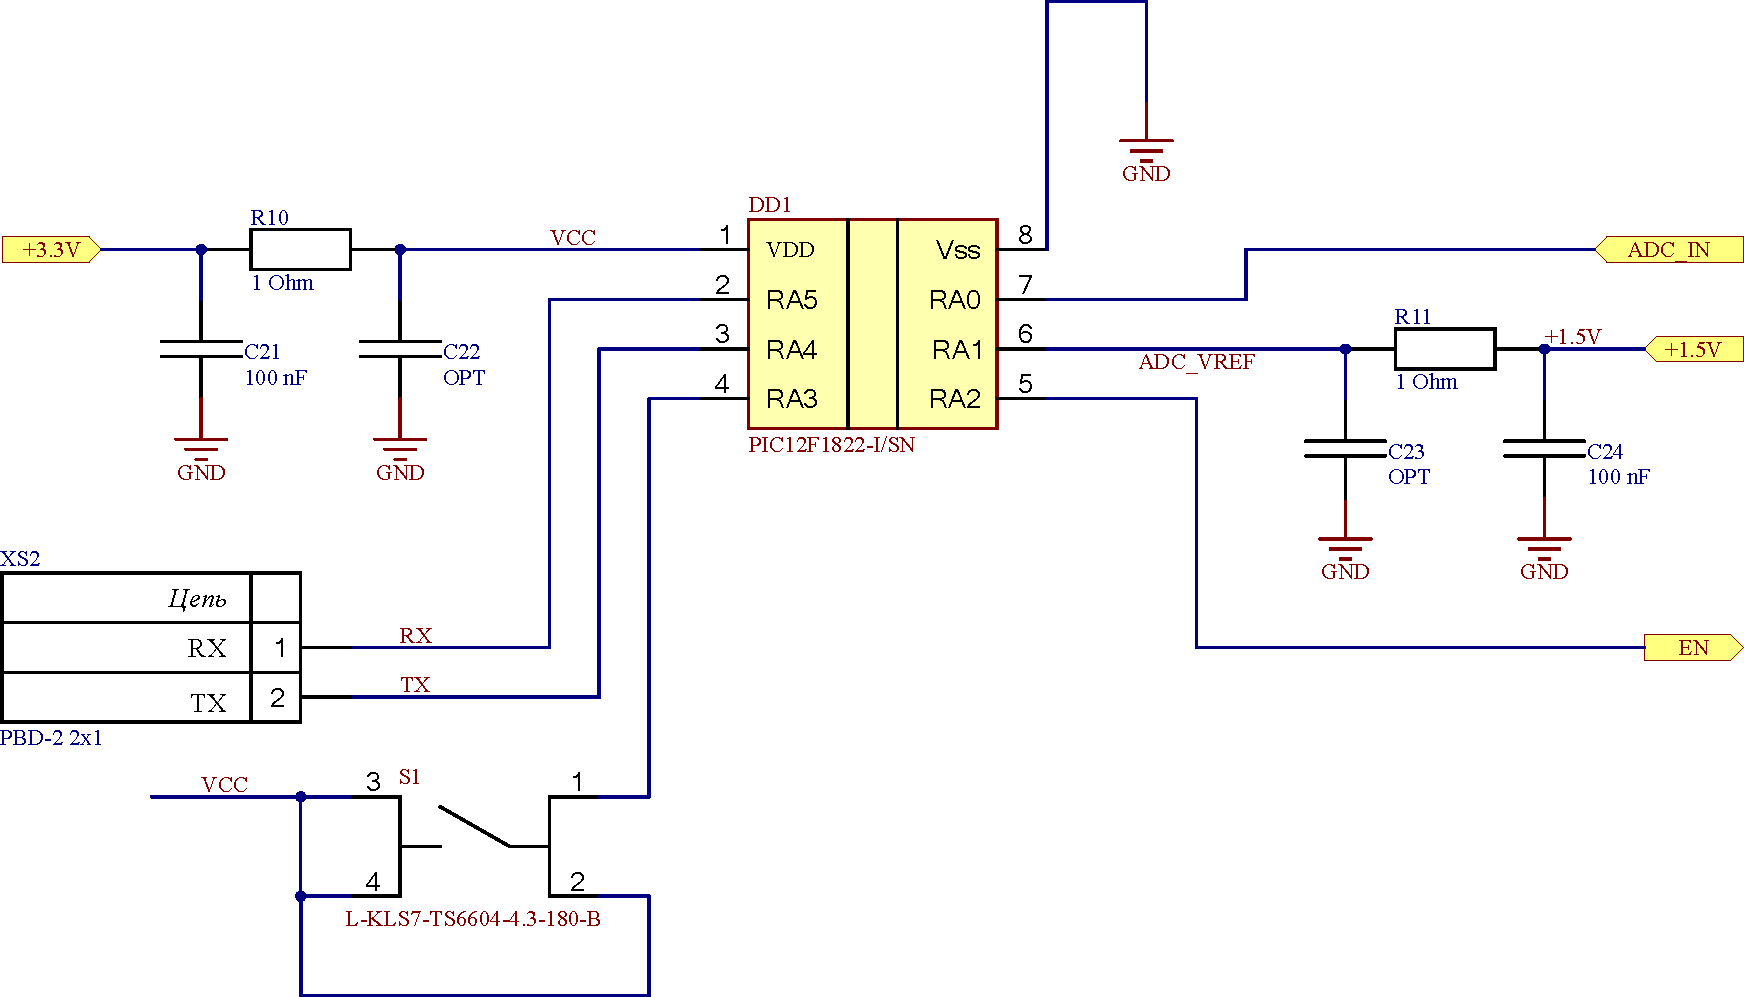
\includegraphics[width=\textwidth, height=0.6\textheight, keepaspectratio]{MC_SchDoc.pdf}	
	\end{frame}
	
\subsection{Подсистема питания}
	
	\begin{frame}
		\frametitle{\insertsection}
		\framesubtitle{\insertsubsection}
		\centering
		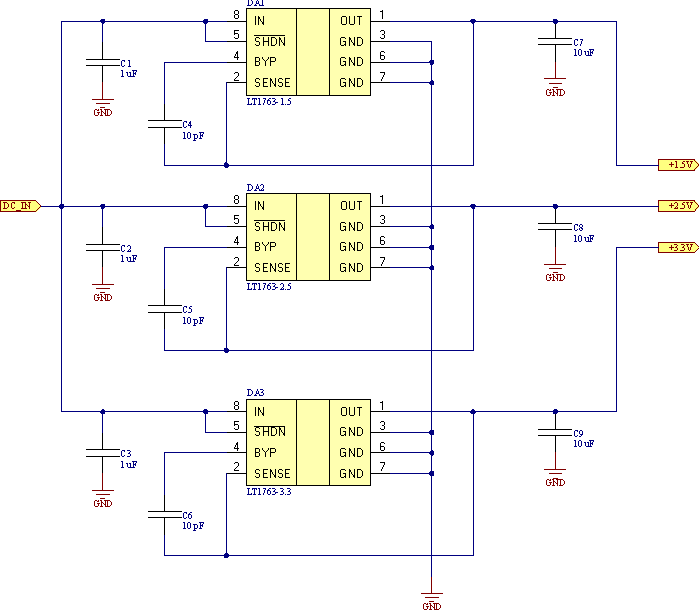
\includegraphics[width=\textwidth, height=0.6\textheight, keepaspectratio]{PM_SchDoc.pdf}	
	\end{frame}

\subsection{Подготовка посадочных мест}

	\begin{frame}
		\frametitle{\insertsection}
		\framesubtitle{\insertsubsection}
		\begin{center}
			\begin{figure}
				\begin{subfigure}[t]{0.5\textwidth}
					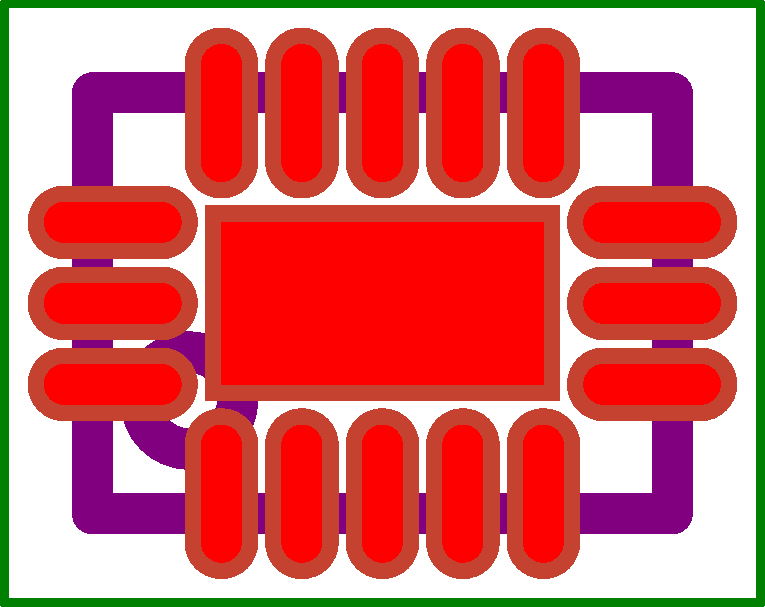
\includegraphics[width=0.9\textwidth, height=0.35\textheight, keepaspectratio]{LNA_PCB_View.pdf}
				\end{subfigure}%
				\begin{subfigure}[t]{0.5\textwidth}
					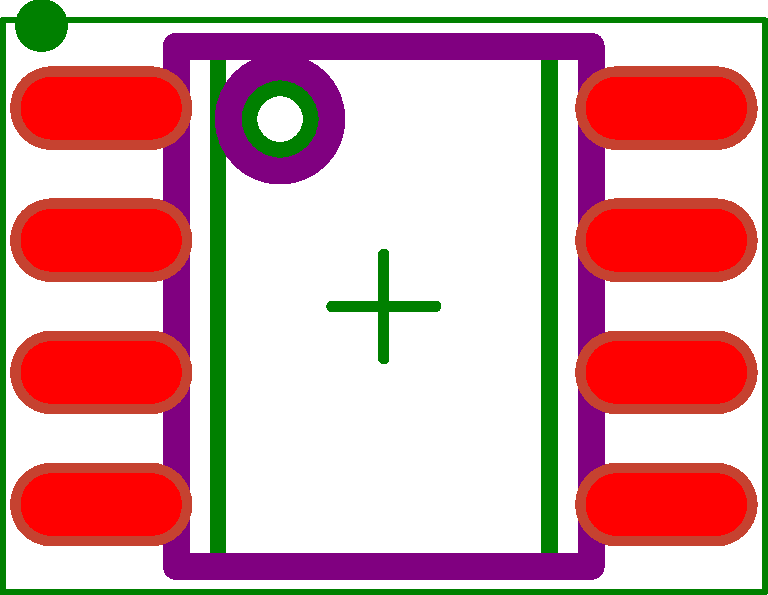
\includegraphics[width=0.9\textwidth, height=0.4\textheight, keepaspectratio, angle=0]{MC_PCB_View.pdf}
				\end{subfigure}
				
				\begin{subfigure}[b]{0.5\textwidth}
					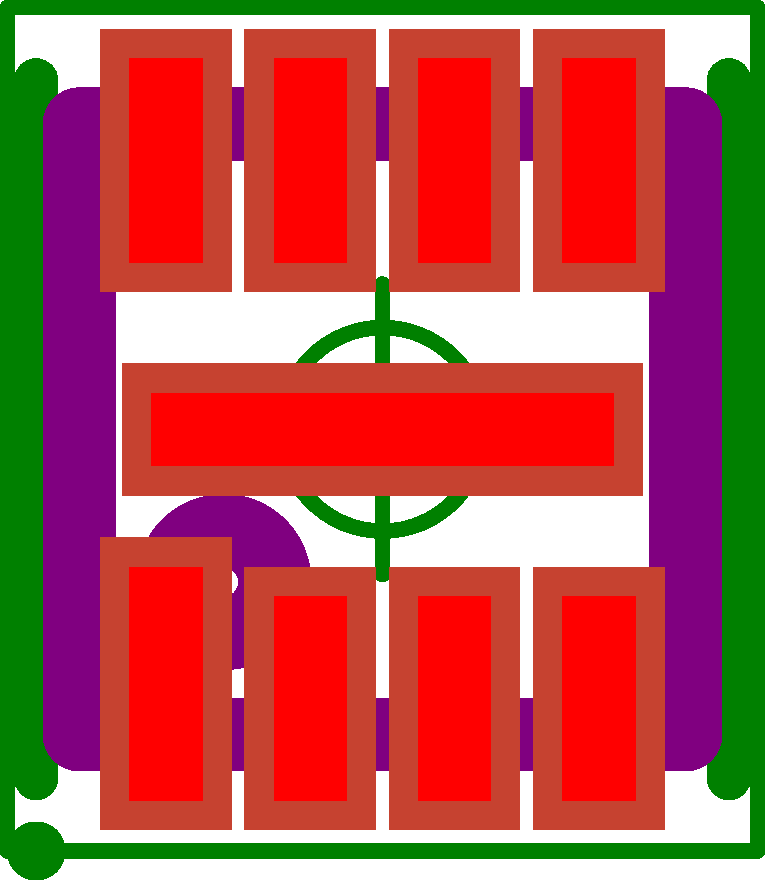
\includegraphics[width=0.9\textwidth, height=0.35\textheight, keepaspectratio, angle=-90]{PD_PCB_View.pdf}
				\end{subfigure}%
				\begin{subfigure}[b]{0.5\textwidth}
					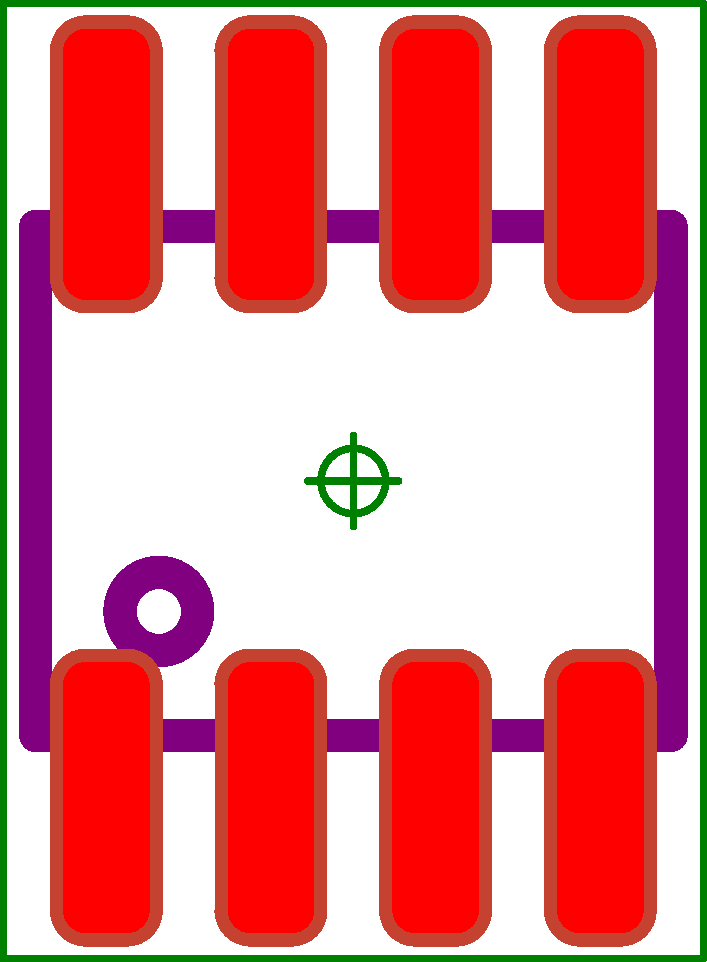
\includegraphics[width=0.9\textwidth, height=0.4\textheight, keepaspectratio, angle=-90]{PM_PCB_View.pdf}
				\end{subfigure}
			\end{figure}
		\end{center}
	\end{frame}

\subsection{Топология}
	
	\begin{frame}
		\frametitle{\insertsection}
		\framesubtitle{\insertsubsection}
		\centering
		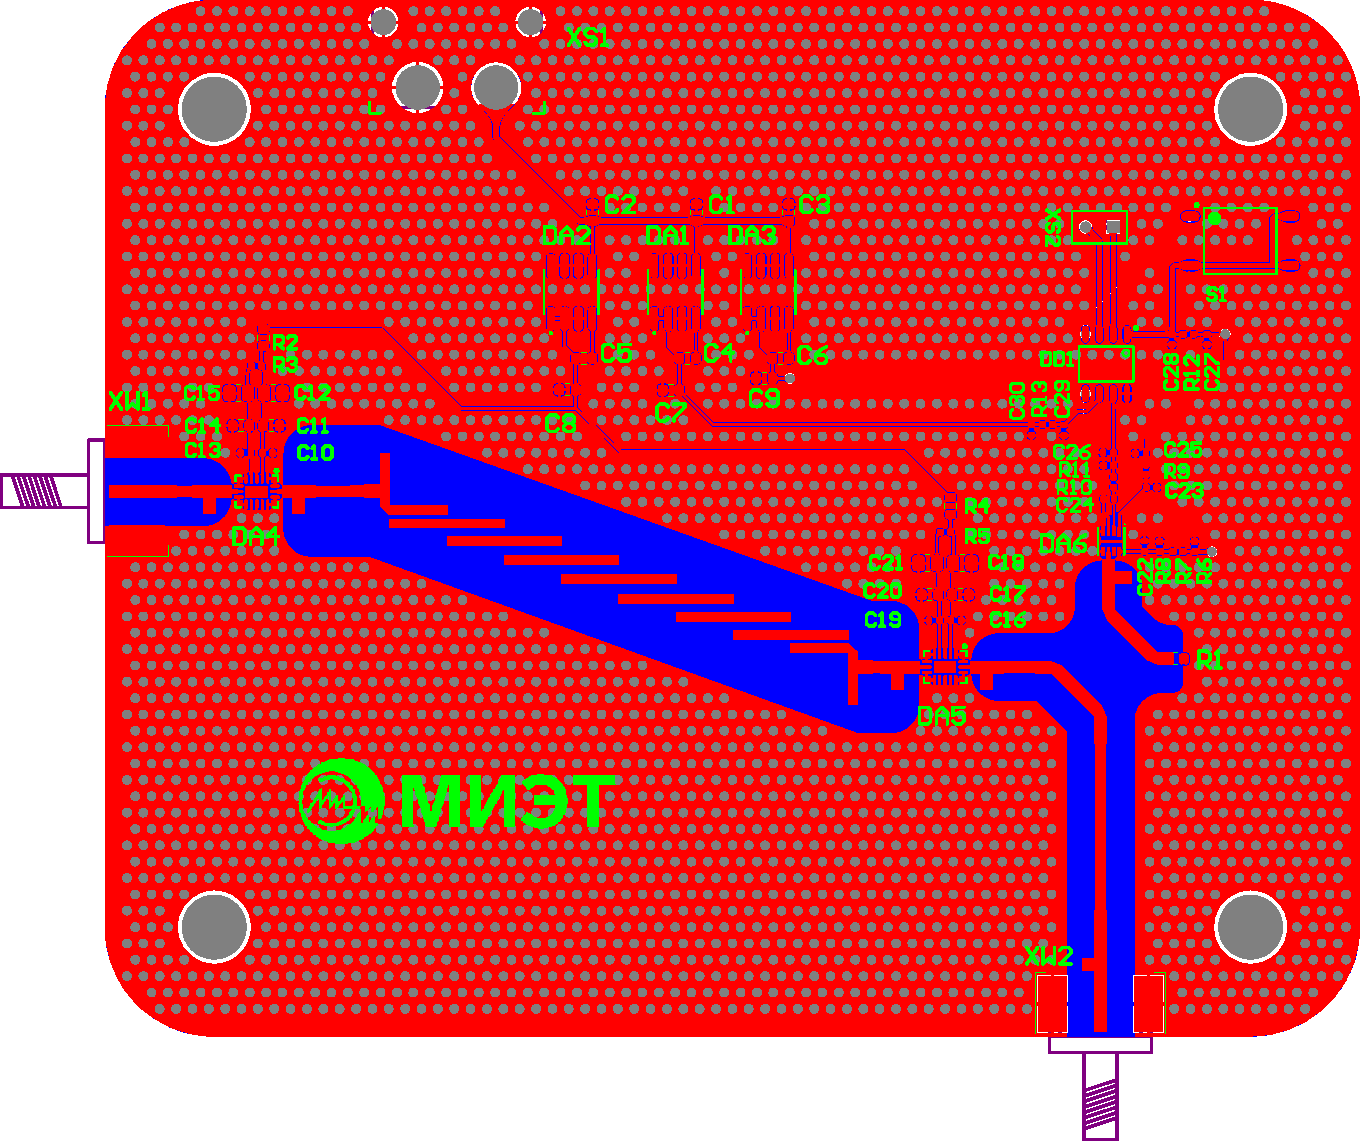
\includegraphics[width=\textwidth, height=0.8\textheight, keepaspectratio]{2LayerAll.pdf}	
		
	\end{frame}

\subsection{Верхний слой}
	
	\begin{frame}
		\frametitle{\insertsection}
		\framesubtitle{\insertsubsection}
		\centering
		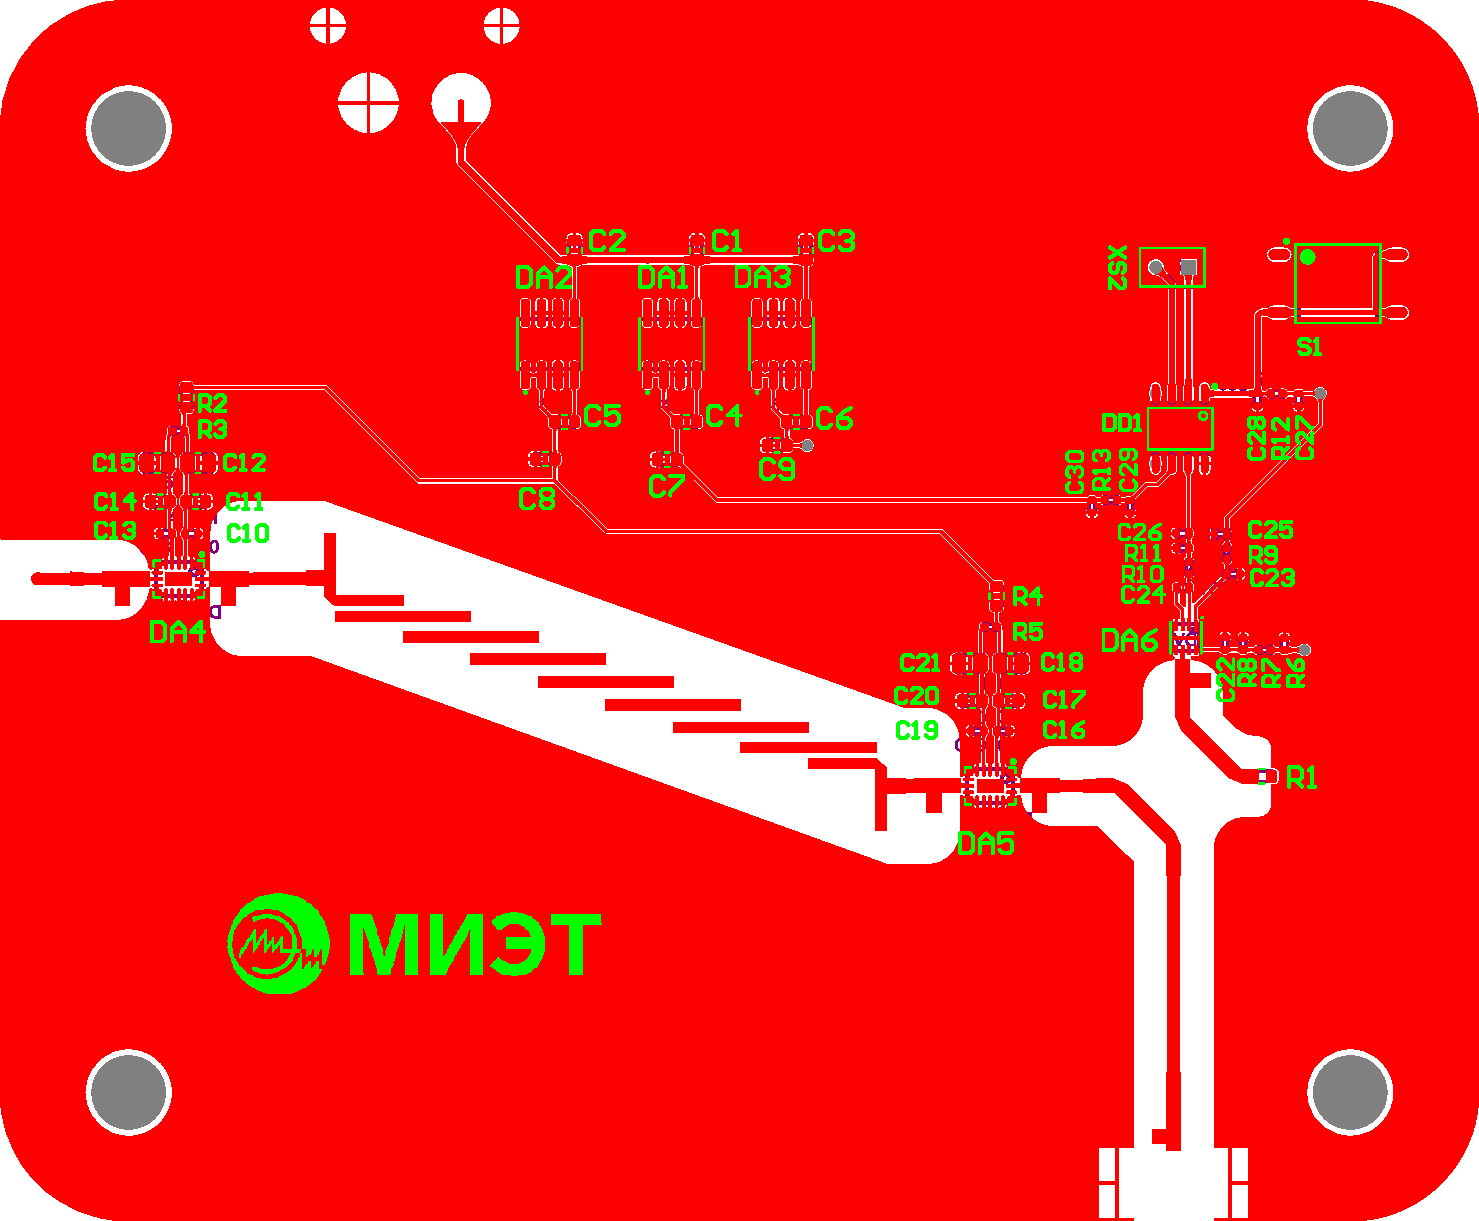
\includegraphics[width=\textwidth, height=0.8\textheight, keepaspectratio]{2LayerTL.pdf}	
		
		
	\end{frame}

\subsection{Нижний слой}
	
	\begin{frame}
		\frametitle{\insertsection}
		\framesubtitle{\insertsubsection}
		\centering
		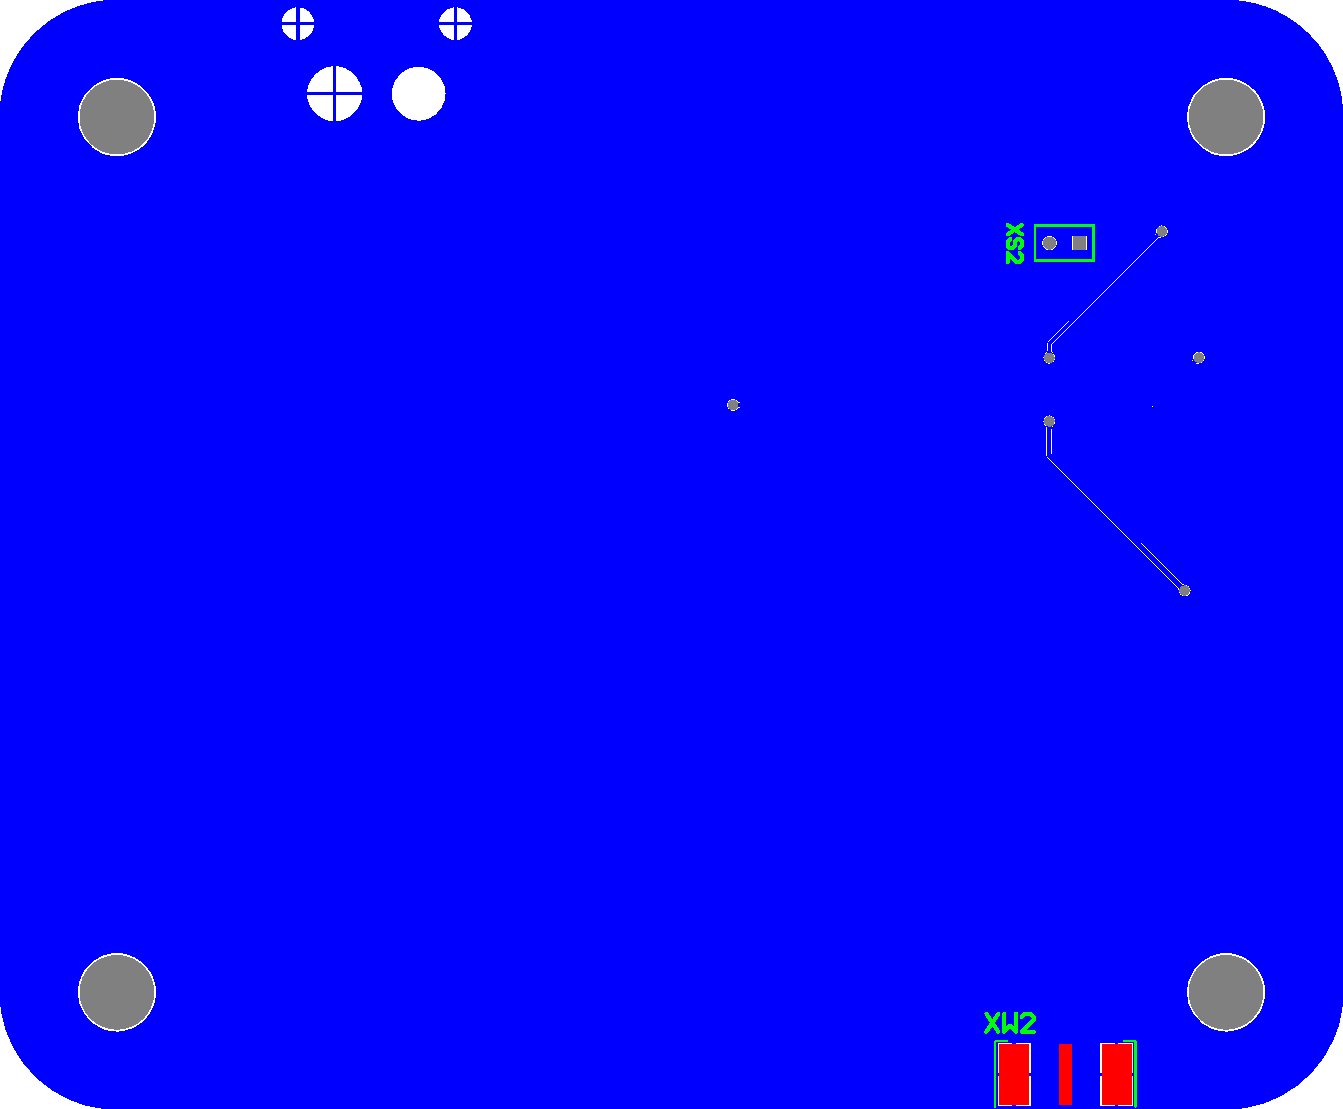
\includegraphics[width=\textwidth, height=0.8\textheight, keepaspectratio]{2LayerBL.pdf}	
		
		
	\end{frame}

\subsection{3D}

	\begin{frame}
		\frametitle{\insertsection}
		\framesubtitle{\insertsubsection}
		\begin{figure}
			\centering\
			\begin{subfigure}{0.5\textwidth}
				\centering
				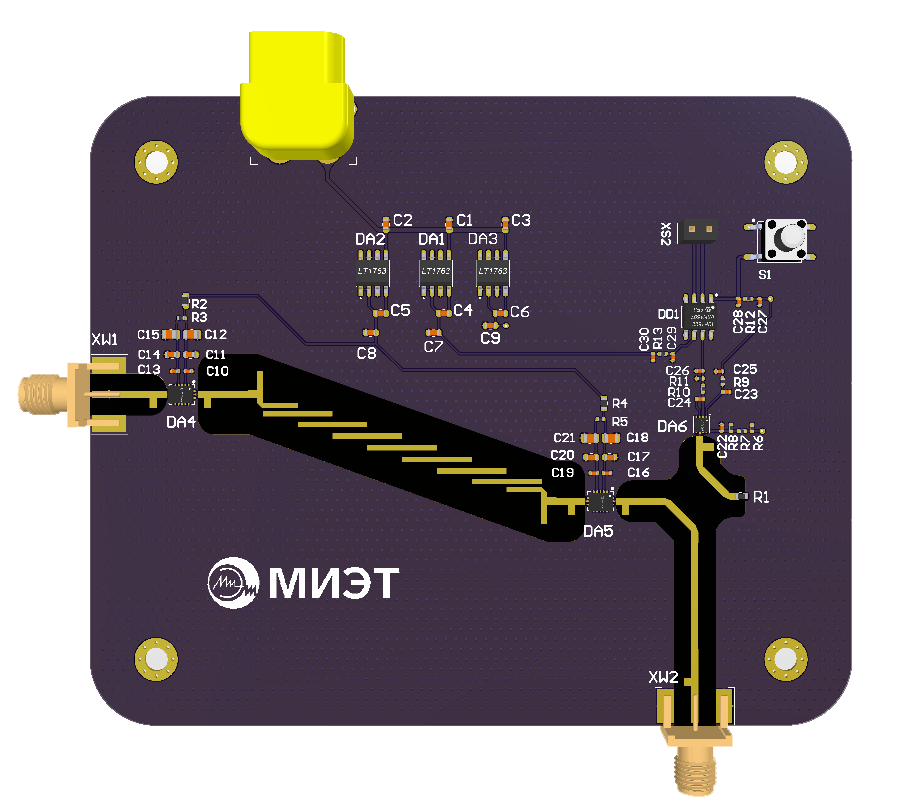
\includegraphics[width=0.98\textwidth]{2Layer1.png}
			\end{subfigure}%
			\begin{subfigure}{0.5\textwidth}
				\centering
				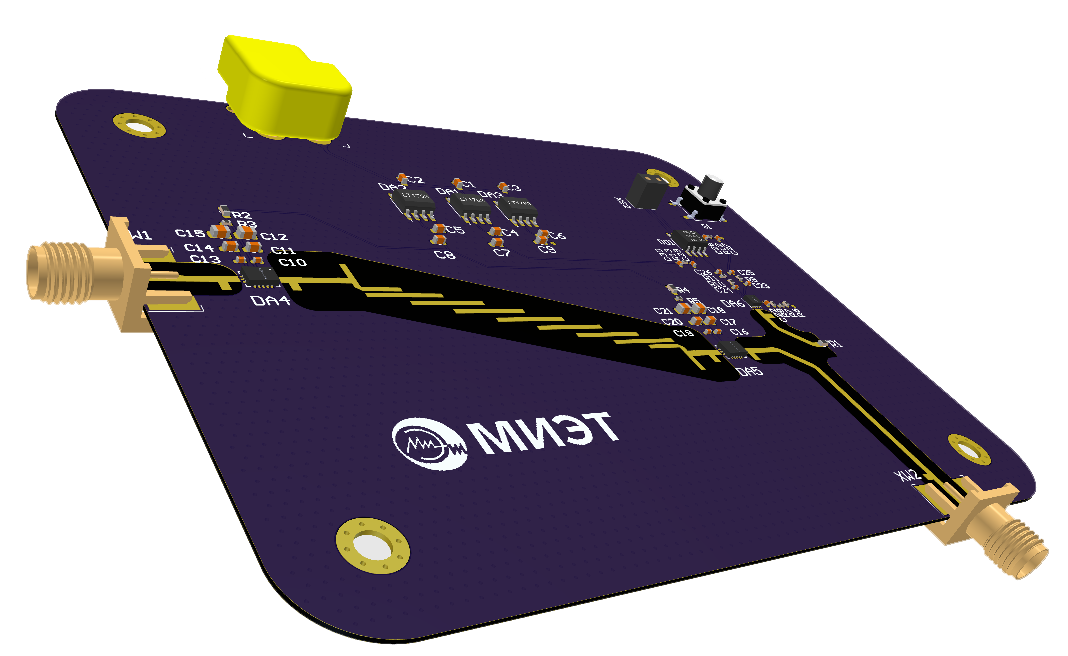
\includegraphics[width=0.98\textwidth]{2Layer0.png}
			\end{subfigure}
		\end{figure}
	\end{frame}

\subsection{Изменения для перехода к корпусному виду}

	\begin{frame}
		\frametitle{\insertsection}
		\framesubtitle{\insertsubsection}
		\centering
		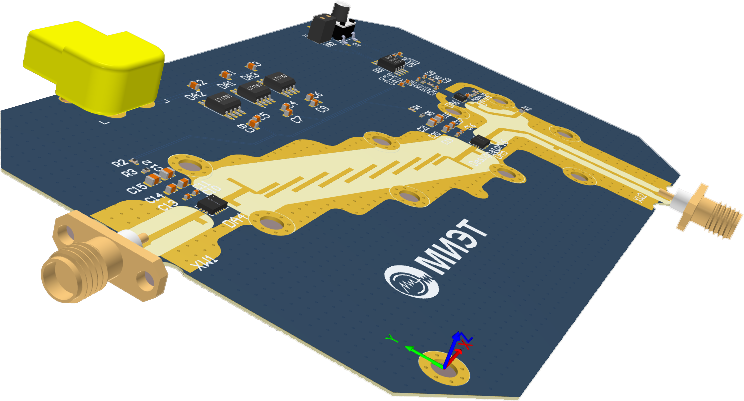
\includegraphics[width=\textwidth, height=0.8\textheight, keepaspectratio]{OpenBoardRelease.png}
	\end{frame}

\section{Дополнительные работы}
\subsection{Плата в корпусе без крышки}
	
	\begin{frame}
		\frametitle{\insertsection}
		\framesubtitle{\insertsubsection}
		\centering
		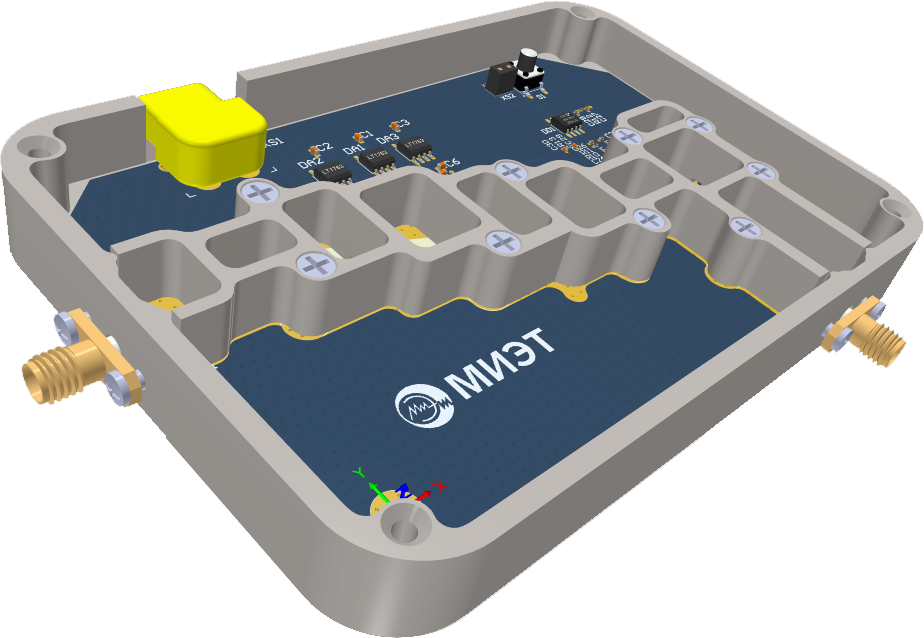
\includegraphics[width=\textwidth, height=0.8\textheight, keepaspectratio]{BoardNoCup.png}		
	\end{frame}

\subsection{Плата в корпусе}

	\begin{frame}
		\frametitle{\insertsection}
		\framesubtitle{\insertsubsection}
		\centering
		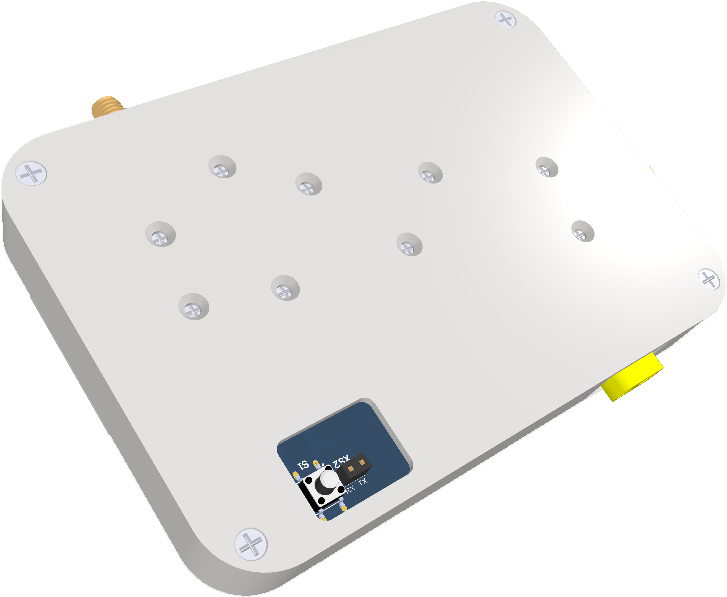
\includegraphics[width=\textwidth, height=0.8\textheight, keepaspectratio]{BoardWithCup.png}		
	\end{frame}

\section{Конструкторская документация}

	
	\begin{frame}
		\frametitle{\insertsection}
		\framesubtitle{\insertsubsection}
		\begin{center}
			\begin{figure}
				%\hspace*{0.1\textwidth}%
				\begin{subfigure}{0.5\textwidth}
					
					\begin{subfigure}[t]{\textwidth}
						\includegraphics[width=\textwidth, height=0.4\textheight, keepaspectratio, page=5]{DocShowOff.pdf}	
					\end{subfigure}
					
					
					\begin{subfigure}[b]{\textwidth}
						\includegraphics[width=\textwidth, height=0.4\textheight, keepaspectratio, page=6]{DocShowOff.pdf}
					\end{subfigure}
					
				\end{subfigure}%
				%
				%
				\begin{subfigure}{0.5\textwidth}
					\begin{subfigure}[t]{\textwidth}
						\includegraphics[width=\textwidth, height=0.4\textheight, keepaspectratio, page=7]{DocShowOff.pdf}
					\end{subfigure}
					
					
					\begin{subfigure}[b]{\textwidth}
						\includegraphics[width=\textwidth, height=0.4\textheight, keepaspectratio, page=8]{DocShowOff.pdf}
					\end{subfigure}
				\end{subfigure}	
			\end{figure}
		\end{center}
	\end{frame}

	\begin{frame}[plain]
		\centering
		\hspace*{-0.1\textwidth}%
		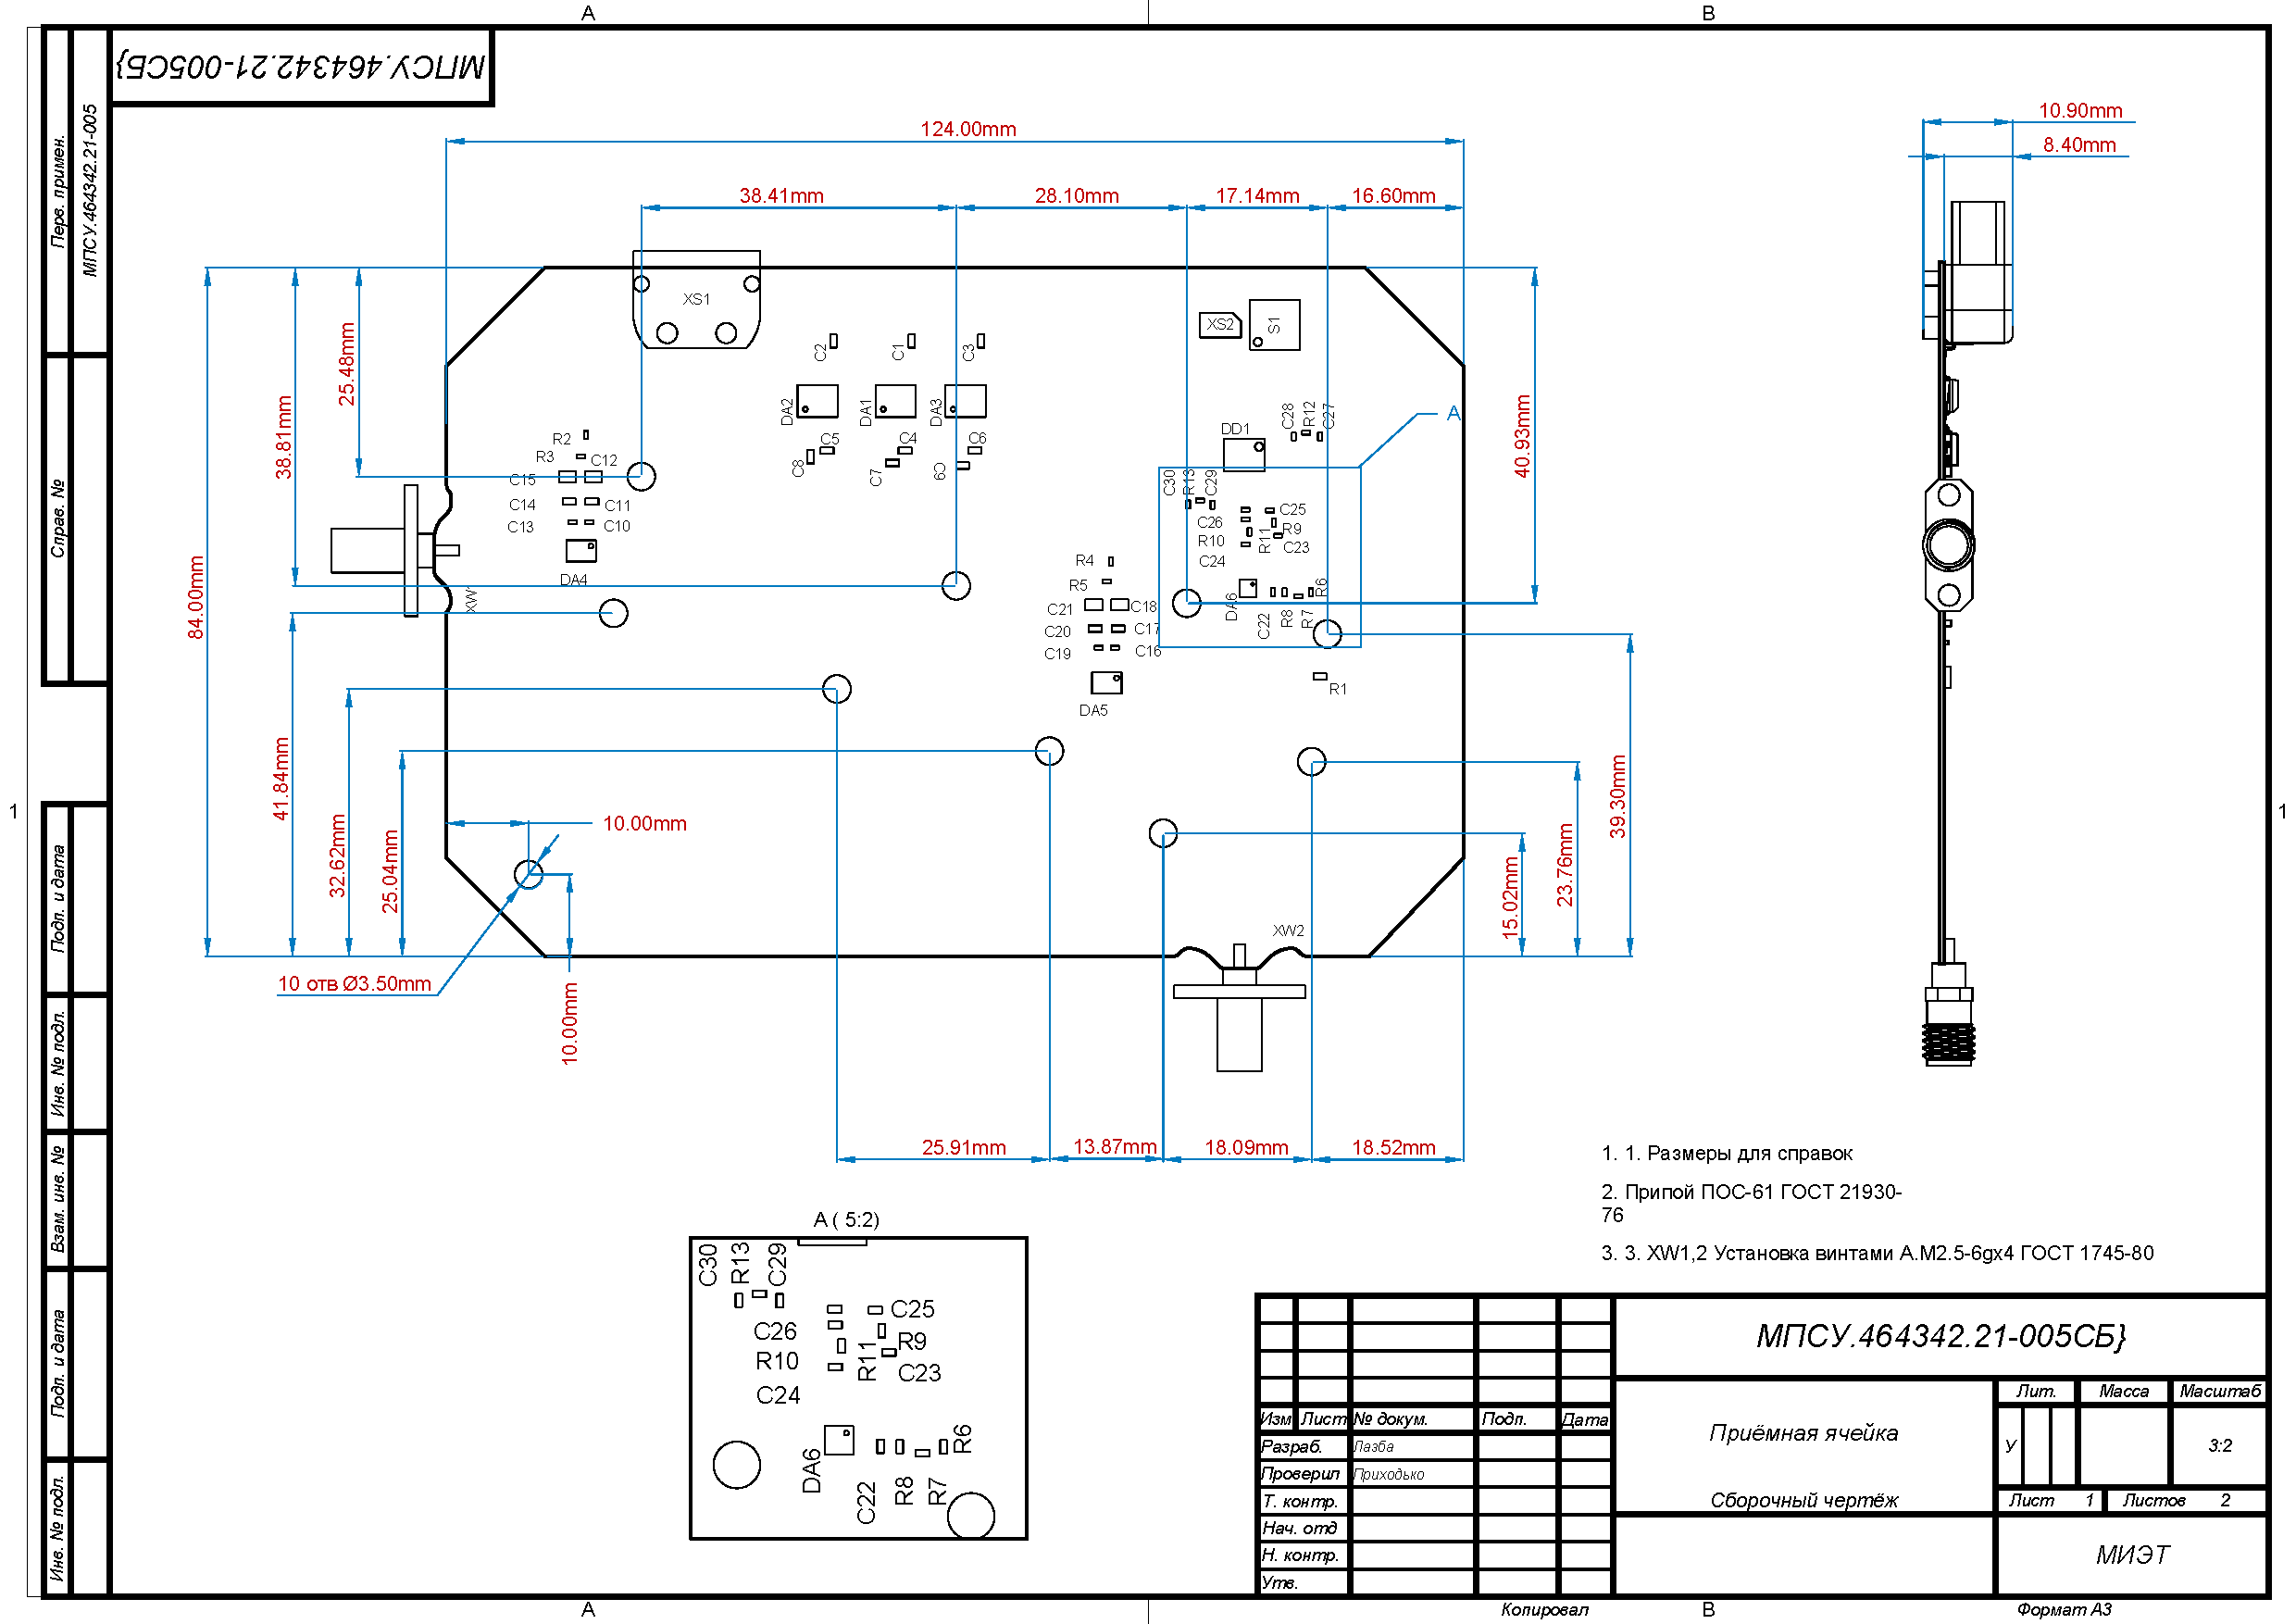
\includegraphics[width=\paperwidth, height=\textheight, keepaspectratio, page=1]{DocShowOff.pdf}
	\end{frame}

	\begin{frame}[plain]
		\centering
		\hspace*{-0.1\textwidth}%
		\includegraphics[width=\paperwidth, height=\textheight, keepaspectratio, page=2]{DocShowOff.pdf}
	\end{frame}

	\begin{frame}[plain]
		\centering
		\hspace*{-0.1\textwidth}%
		\includegraphics[width=\paperwidth, height=\textheight, keepaspectratio, page=3]{DocShowOff.pdf}
	\end{frame}

	\begin{frame}[plain]
		\centering
		\hspace*{-0.1\textwidth}%
		\includegraphics[width=\paperwidth, height=\textheight, keepaspectratio, page=4]{DocShowOff.pdf}
	\end{frame}

	\begin{frame}[plain]
		\centering
		\hspace*{-0.1\textwidth}%
		\includegraphics[width=\paperwidth, height=\textheight, keepaspectratio, page=9]{DocShowOff.pdf}
	\end{frame}

	\begin{frame}[plain]
		\centering
		\hspace*{-0.1\textwidth}%
		\includegraphics[width=\paperwidth, height=\textheight, keepaspectratio, page=10]{DocShowOff.pdf}
	\end{frame}


	\begin{frame}
		\frametitle{Спасибо за внимание!}
		\framesubtitle{Спасибо за внимание!}
		\centering \Huge Спасибо за внимание!		
	\end{frame}
\end{document}